\documentclass[11pt,a4paper]{report}

\usepackage[utf8]{inputenc}
\usepackage{booktabs}
\usepackage{graphicx}
\usepackage{amsmath,amssymb}
\usepackage{geometry}
\usepackage{fancyhdr}
\usepackage{hyperref}
\usepackage{float}
\usepackage{setspace}
\usepackage{eso-pic}
\usepackage{xcolor}

\geometry{
    left=1in,
    right=1in,
    top=1in,
    bottom=1in
}

\pagestyle{fancy}
\setlength{\headheight}{14pt}
\fancyhf{}
\fancyhead[L]{\nouppercase{\leftmark}}
\fancyhead[R]{\thepage}

\setstretch{1.15}

\title{\Huge \textbf{} \\[0.5em]\large}
\author{}
\date{}

\begin{document}

\AddToShipoutPictureBG*{%
    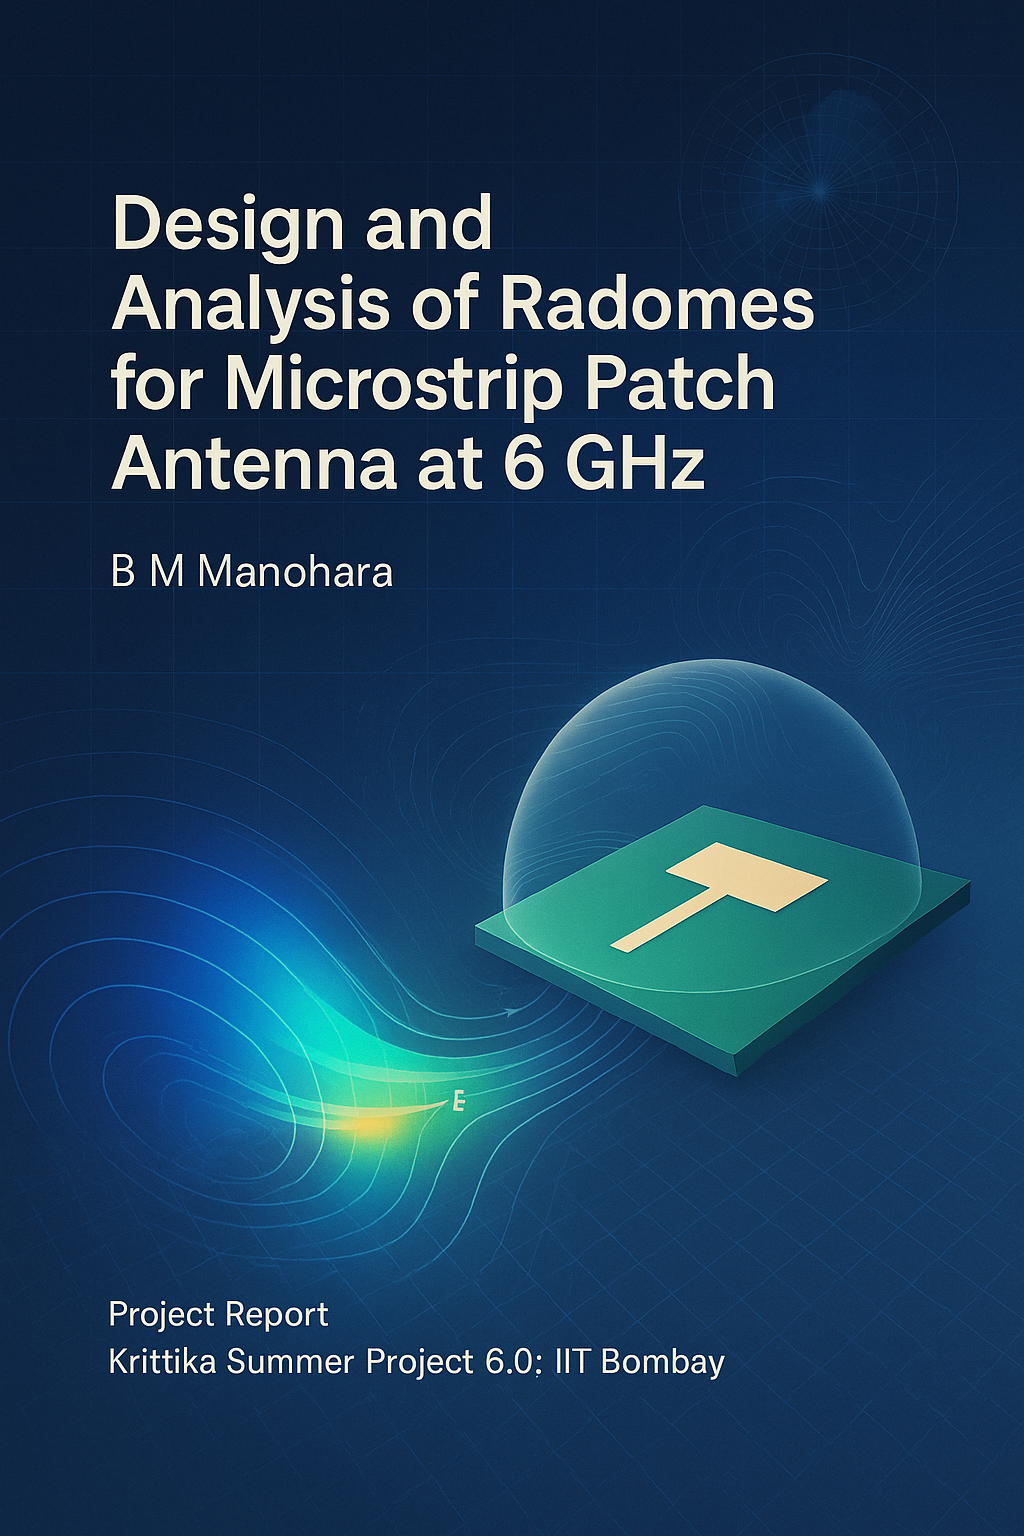
\includegraphics[width=\paperwidth,height=\paperheight]{figures/cover1.png}%
}

\maketitle

% Second page blank after title
\cleardoublepage
\thispagestyle{empty}
\null
\newpage

\chapter*{Title Page}
\addcontentsline{toc}{chapter}{Title Page}
\thispagestyle{empty}

\vspace*{2cm}
{\Large \textcolor{orange}{\textbf{KRITTIKA SUMMER PROJECTS 2025}} \par}
\vspace{1cm}
{\Huge \bfseries \textcolor{red}{Design and Analysis of Radomes} \par}
\vspace{0.2cm}
{\Huge \bfseries \textcolor{red}{for Microstrip Patch Antenna} \par}
\vspace{0.2cm}
{\Huge \bfseries \textcolor{red}{at 6GHz} \par}
\vspace{1.5cm}
{\large \textbf{\textcolor{olive}{B M Manohara}} \par}
\vspace{1.5cm}

\begin{flushleft}
1. Krittika-The Astronomy Club of IIT Bombay, Powai, Mumbai 400076, India \\
2. R V College Of Engineering, Bengaluru, Karnataka 560059, India \\
3. Dhruva-The Astronomy Club of RVCE, Bengaluru, Karnataka 560059, India
\end{flushleft}

\vfill
\begin{flushleft}
\footnotesize
\textcopyright{} 2025 Krittika IITB \\
    \textbf{Published by Krittika: The Astronomy Club of IIT Bombay} \\[0.5em]
    \href{https://github.com/krittikaiitb}{github.com/krittikaiitb} \\
    \href{https://github.com/Manohara-Ai}{github.com/Manohara-Ai} \\
    Repository: \texttt{Design\_and\_Analysis\_of\_Flat\_Radomes\_for\_MSPA} \\[0.5em]
    First Release, August 2025
\end{flushleft}

\cleardoublepage
\thispagestyle{empty}
\null
\newpage

\chapter*{Abstract}

Astronomy experiments operating at radio frequencies (RF) and higher are rapidly growing in both scale and importance. Observations in these spectral regions enable us to explore fundamental questions, from tracing the thermal history of the universe to studying the conditions present during the early stages of universe. Antennas operating at these wavelengths, typically in the millimeter scales, are often cooled to cryogenic temperatures to reduce thermally generated noise. To maintain a vacuum environment around such antennas, protective radome structures are used. However, these radomes can distort the antenna’s beam pattern, potentially degrading the quality and integrity of the observations. As the operating frequency decreases toward longer radio wavelengths, the required radome thickness increases, introducing additional signal losses.

In this work, we design a range of antennas operating at mspa millimeter wavelengths, enclose them within flat radome structure, and carry out a detailed analysis of the antenna–radome system. Ultimately, this study aims to identify positioning strategies that minimize signal degradation and preserve the integrity of the antenna radiation pattern.

\tableofcontents
\listoffigures
\listoftables

% Chapters split in separate files
\cleardoublepage
\thispagestyle{empty}
\null
\newpage

\chapter{Introduction}

The rapid growth of wireless communication, satellite systems, and high-frequency radio astronomy experiments has created an increasing demand for compact, efficient, and cost-effective antenna solutions. Microstrip patch antennas have become highly attractive candidates due to their low profile, ease of fabrication, and compatibility with modern printed circuit technologies \cite{werfelli2016patch,balanis}. These antennas are well-suited for integration in arrays and conformal platforms, supporting applications ranging from telecommunications to scientific observation.

However, microstrip patch antennas are sensitive to their surrounding environment. Environmental factors such as rain, wind, dust, or mechanical impacts can degrade antenna performance or even cause damage. To overcome these challenges, antennas are typically housed within protective structures known as radomes. A radome is a structural, weatherproof enclosure that shields the antenna while aiming to minimally affect its electromagnetic performance \cite{swra705,aemterms}. Ideally, a radome should be transparent to the antenna’s operating frequency, maintaining the integrity of the radiation pattern and minimizing losses.

In radio astronomy applications, where extremely high sensitivity is required, the impact of radomes becomes even more critical. Subtle distortions introduced by the radome can affect beam shapes, sidelobe levels, or polarization purity, thereby impacting the accuracy of scientific measurements \cite{mcculloch2023sband}. Moreover, as the operating frequency decreases toward radio wavelengths, the radome’s physical thickness increases to maintain structural integrity, which may result in additional signal attenuation or pattern distortion.

This project focuses on understanding the design principles of patch antennas and analyzing the effect of various radome configurations on antenna performance. Building on the foundation of electromagnetic radiation theory \cite{balanis}, the project will explore flat, spherical, and other radome geometries through simulation. The ultimate goal is to identify suitable radome materials and shapes that protect the antenna while preserving its desired electromagnetic characteristics.

\section*{Conclusion}

This introductory chapter outlined the motivation behind studying radome-antenna interactions in RF systems, particularly in the context of radio astronomy. It also introduced the challenges posed by environmental effects on high-frequency antennas and the need for careful radome design. With this context, the next chapter builds the theoretical foundation of antenna radiation, laying the groundwork for simulation and analysis.

\chapter{Theory of Antenna Radiation}

\section{Radiation from a Conducting Rod}

A simple metallic rod can radiate electromagnetic energy when an alternating current (AC) is applied to it. The mechanism of radiation is fundamentally tied to the time-varying current along the conductor. Oscillating electrons within the rod generate a time-varying current, producing a time-varying electric field. According to Maxwell’s equations, this changing electric field creates a magnetic field, resulting in a propagating electromagnetic wave. A uniform, steady current will not radiate, whereas a current with spatial and temporal variation will. When the length of the rod is approximately half the wavelength of the incoming electric field, it becomes an efficient radiator, forming the well-known half-wave dipole.

\section{Transmission Lines and Directed Radiation}

Transmission lines, such as coaxial cables or parallel-wire lines, are engineered to transport electromagnetic energy with minimal loss while avoiding radiation. When the end of a transmission line is modified to open into free space, as in the case of a horn antenna, it can serve as a directional radiator. A horn antenna achieves this by gradually flaring the transmission line to match the impedance of free space.

\section{Dipole Antennas}

A dipole antenna consists of two conductive arms aligned end-to-end with a small feed gap. The alternating current through the arms produces radiated electromagnetic fields. The resulting pattern is typically doughnut-shaped, with maximum radiation perpendicular to the dipole axis and nulls along its length. For a half-wave dipole, each arm has length $\lambda/4$, giving a total dipole length of $\lambda/2$. The radiated power is described by the Poynting vector:
\[
\vec{S} = \vec{E} \times \vec{H}
\]
which represents the flow of electromagnetic energy away from the antenna.

\begin{figure}[H]
    \centering
    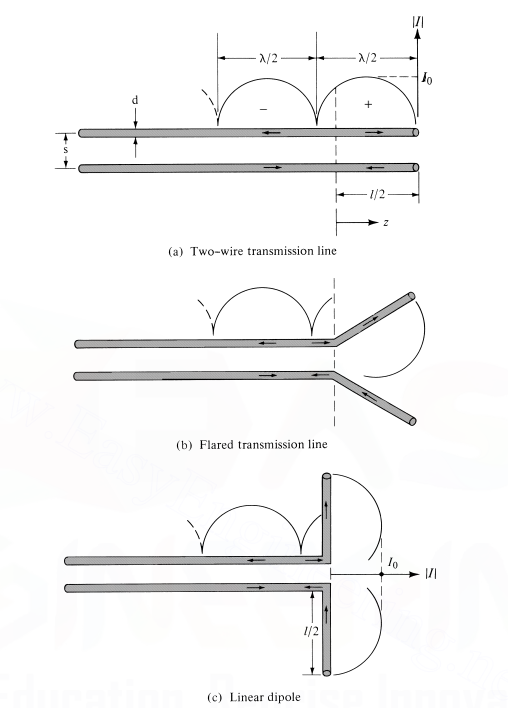
\includegraphics[width=0.75\textwidth]{figures/dipole.png}
    \caption{Current distribution on a lossless two-wire transmission line, flared transmission line, and linear dipole.}
    \small Image adapted from \cite{balanis}.
    \label{fig:dipole-current}
\end{figure}

\section{Isotropic Antennas and Radiation Parameters}

An isotropic antenna is a hypothetical point source that radiates equally in all directions, used as a reference for comparing real antennas. Its associated parameters include:

\begin{itemize}
    \item \textbf{Radiation intensity:}
    \[
    U(\theta,\phi) = r^2 S_r(\theta,\phi)
    \]
    where $S_r$ is the radial component of the Poynting vector.
    \item \textbf{Total radiated power:}
    \[
    P_{rad} = \int_{0}^{2\pi} \int_{0}^{\pi} U(\theta,\phi) \sin\theta \, d\theta \, d\phi
    \]
\end{itemize}

\section{Radiation Patterns and Beam Characteristics}

An antenna’s radiation pattern describes the spatial distribution of radiated power, typically represented in polar or 3D plots. These patterns help visualize how the antenna emits or receives energy in various directions.

Key features of a radiation pattern include:

\begin{itemize}
    \item \textbf{Main lobe}: The region of the radiation pattern that contains the direction of maximum radiation. This is typically aligned with the antenna’s boresight—defined as the axis or direction in which the antenna radiates most strongly.
    
    \item \textbf{Side lobes}: Smaller lobes that occur in directions away from the main beam. These represent unwanted radiation that can cause interference or reduce antenna efficiency.
    
    \item \textbf{Back lobe}: A specific side lobe that appears opposite to the main lobe, often minimized in directional antennas.
    
    \item \textbf{Nulls}: Directions in which the radiated power drops to zero or a local minimum. These are useful in applications like interference suppression or direction finding.
\end{itemize}

The \textbf{boresight} refers to the central axis of the main lobe—usually orthogonal to the plane of a symmetric antenna such as a dipole or horn. Beam steering, alignment, and antenna performance are often evaluated with respect to the boresight direction.

Radiation patterns can be analyzed by measuring or computing the far-field electromagnetic fields produced by the antenna. For electrically small antennas or arrays, Fourier transforms of the current distribution are commonly used to derive the angular power distribution.

\begin{figure}[H]
    \centering
    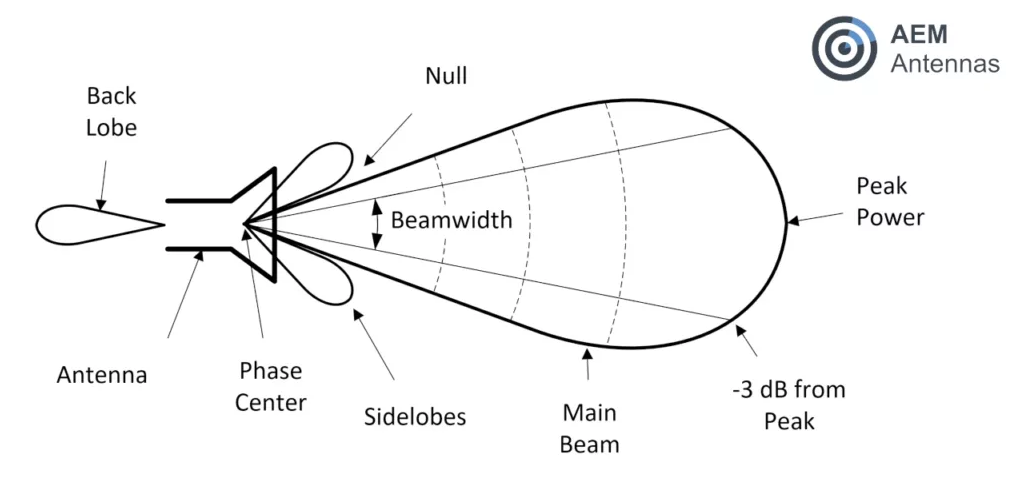
\includegraphics[width=0.7\textwidth]{figures/lobe.png}
    \caption{Visualization of an antenna radiation pattern showing the main lobe, side lobes, back lobe, and nulls.\\[0.5em]
    \small Image adapted from \cite{aemterms}.}
    \label{fig:lobes-pattern}
\end{figure}

\section{Beamwidth and Bandwidth}

Key parameters describing antennas include:
\begin{itemize}
    \item \textbf{HPBW (Half Power Beam Width)}:
    \[
    \theta_{HPBW} = \theta_2 - \theta_1, \quad \text{where } U(\theta_{1,2}) = 0.5 U_{max}
    \]
    \item \textbf{FNBW (First Null Beam Width)}: the angular separation between the first nulls on each side of the main lobe
\end{itemize}

\section{Gain and Directivity}

\begin{itemize}
    \item \textbf{Directivity}:
    \[
    D = \frac{4\pi U_{max}}{P_{rad}}
    \]
    \item \textbf{Gain}:
    \[
    G = \eta D
    \]
    where $\eta$ is the radiation efficiency, incorporating conductor or dielectric losses.
\end{itemize}

\section{S-Parameters in Antenna Design}

In RF analysis, antennas are treated as ports in a network. The reflection coefficient $S_{11}$ describes how much of the incident power is reflected:
\[
S_{11} = \frac{V_{reflected}}{V_{incident}}
\]
A value of $S_{11}$ below $-10\,\mathrm{dB}$ is generally considered acceptable.

\begin{figure}[H]
    \centering
    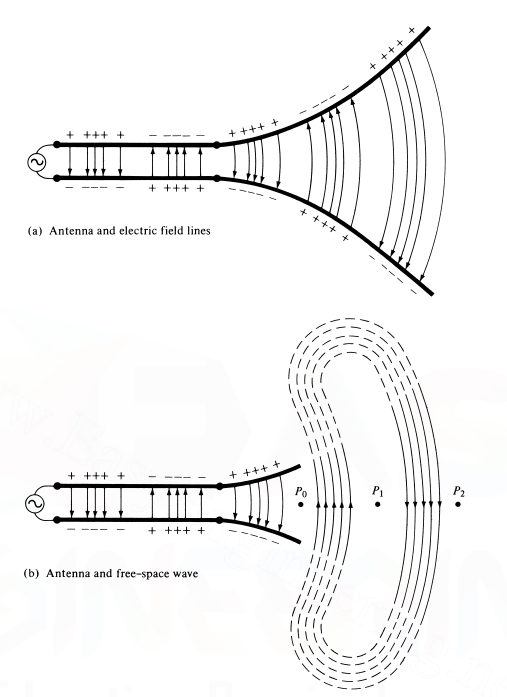
\includegraphics[width=0.6\textwidth]{figures/radiation.png}
    \caption{Source, transmission line, antenna, and detachment of electric field lines.}
    \small Image adapted from \cite{balanis}.
    \label{fig:radiation-overview}
\end{figure}

\section*{Conclusion}

This chapter provided a foundational understanding of antenna radiation by examining how time-varying currents generate electromagnetic fields and propagate energy through space. Key models such as dipole antennas and isotropic radiators were discussed, along with critical performance metrics including gain, directivity, beamwidth, and impedance characteristics.

While these theoretical principles help in designing efficient antennas under ideal conditions, real-world environments often introduce factors—such as weather, dust, or mechanical stress—that degrade antenna performance. This leads to the need for protective enclosures that can preserve radiation characteristics while shielding the antenna from external conditions.

In the next chapter, we introduce radomes: dielectric structures designed to protect antennas while maintaining electromagnetic transparency. We explore how their material properties, geometry, and placement can significantly impact the radiation behavior of enclosed antennas.


\chapter{Radomes}

\section{Introduction to Radomes}

A radome (short for “radar dome”) is an electromagnetic enclosure that protects antennas from environmental factors such as wind, rain, dust, temperature fluctuations, and physical damage. While offering mechanical protection, a well-designed radome must remain electromagnetically transparent, ensuring minimal degradation of antenna performance in terms of gain, beam shape, or impedance matching.

Radomes are especially critical in radar, aerospace, and radio astronomy systems, where precise radiation characteristics and consistent long-term operation are required. Improperly chosen radome parameters can lead to signal attenuation, beam distortion, and multipath reflections.

\section{Material Considerations}

An ideal radome material exhibits the following characteristics:

\begin{itemize}
    \item Low relative permittivity ($\varepsilon_r$) — reduces phase delay and impedance mismatch
    \item Low dielectric loss tangent ($\tan\delta$) — minimizes absorption
    \item High mechanical durability and environmental resistance
    \item Stable performance over temperature and frequency variations
\end{itemize}

Common radome materials include PTFE (Teflon), ABS, polycarbonate, and PMMA (Plexiglass). The material used in this study is PMMA, with $\varepsilon_r = 2.8$ and $\tan\delta = 0.001$ at 6~GHz.

\section{Electromagnetic Theory of Radomes}

\subsection*{i. Transmitted and Reflected Wave Behavior}

When an EM wave encounters a dielectric slab (the radome wall), it experiences partial transmission and reflection. The reflection coefficient $\Gamma$ at the air–radome interface is given by:

\[
\Gamma = \frac{\sqrt{\varepsilon_r} - 1}{\sqrt{\varepsilon_r} + 1}
\]

The transmitted wave continues through the radome material with a different wavelength, experiencing phase shift. Multiple reflections inside the slab can constructively or destructively interfere depending on thickness and incident angle.

To minimize reflections and phase distortion, **transmission line analogy** is used. The dielectric slab acts like a transmission line segment of impedance $Z_m = \frac{Z_0}{\sqrt{\varepsilon_r}}$, where $Z_0$ is the impedance of free space.

\subsection*{ii. Optimal Distance Between Antenna and Radome}

The separation between the antenna and radome wall should be carefully selected to prevent standing wave formation and phase errors caused by internal reflections. An optimal distance $D$ satisfies the condition:

\[
D_{\text{opt}} = n \cdot \frac{\lambda_0}{2}, \quad n \in \mathbb{Z}^+
\]

where $\lambda_0$ is the free-space wavelength. At these distances, reflected waves from the radome re-enter the antenna in-phase, minimizing destructive interference.

\subsection*{iii. Optimal Radome Wall Thickness}

To minimize reflections at the radome wall, the thickness $t$ should satisfy the **half-wave matching condition** in the radome material:

\[
t_{\text{opt}} = n \cdot \frac{\lambda_0}{2\sqrt{\varepsilon_r}}, \quad n \in \mathbb{Z}^+
\]

This ensures that reflected waves inside the radome destructively interfere, reducing the effective reflection seen by the antenna. For instance, at 6~GHz and $\varepsilon_r = 2.8$, $\lambda_0 = 50~\mathrm{mm}$, leading to an optimal thickness of approximately:

\[
t \approx \frac{50}{2 \cdot \sqrt{2.8}} \approx 14.95~\mathrm{mm}
\]

for $n = 1$.

\subsection*{iv. Errors Introduced by Flat Radomes}

Flat radomes are simple to manufacture but introduce angular-dependent errors due to refraction and differential phase delay. Key error sources include:

\begin{itemize}
    \item \textbf{Beam broadening or squinting}: Radiation pattern shifts due to phase mismatch.
    \item \textbf{Ripple in gain pattern}: Standing waves between antenna and inner wall.
    \item \textbf{Side lobe distortion}: Especially for wider beams or off-axis rays.
    \item \textbf{Frequency sensitivity}: Optimal thickness and spacing vary with frequency.
\end{itemize}

These errors worsen at large incidence angles and are minimized by curvature-matched (e.g., spherical or conical) radomes in high-precision applications.

\begin{figure}[H]
    \centering
    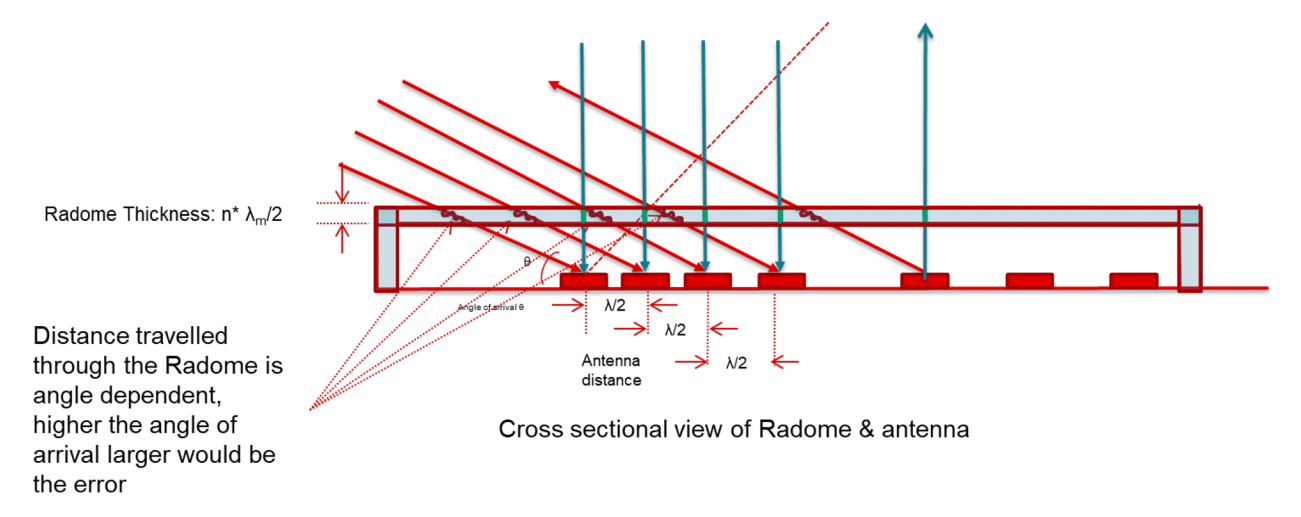
\includegraphics[width=0.9\textwidth]{figures/flat.png}
    \caption{Distance Traveled in Rectangular Radome Wall for Different Grazing Angles.}
    \small Image adapted from \cite{swra705}.
    \label{fig:radome-grazing-angle}
\end{figure}

\section{Design Summary}

To ensure optimal performance:

\begin{itemize}
    \item Select low-loss, low-permittivity materials (e.g., PMMA, PTFE)
    \item Match radome thickness to a multiple of half-wavelength in the material
    \item Set antenna-to-radome spacing to avoid phase error from internal reflections
    \item Consider the operating frequency range and beamwidth in the design
\end{itemize}

These considerations enable the radome to function as a passive, protective structure without compromising the electromagnetic integrity of the antenna system.

\section*{Conclusion}

This chapter explored the function, design parameters, and electromagnetic impact of radomes. Key derivations included reflection coefficients, optimal wall thickness, and antenna-to-radome spacing. Flat radomes, while practical, were shown to introduce beam distortion and phase errors if improperly designed. These theoretical insights will now be applied in the following chapter, where we focus on modeling the microstrip patch antenna to be enclosed by such radomes.

\chapter{Microstrip Patch Antennas}

\section{Structure and Working of Microstrip Patch Antennas}

Microstrip Patch Antennas (MSPAs) are planar antennas widely used in modern wireless systems due to their low profile, ease of fabrication, and compatibility with printed circuit technologies. The basic structure consists of:

\begin{itemize}
    \item A conducting \textbf{patch} (typically rectangular or circular) on the top surface.
    \item A \textbf{dielectric substrate} in the middle.
    \item A continuous \textbf{ground plane} at the bottom.
\end{itemize}

The patch is usually made of copper or gold, and the substrate can be materials like FR4, RT Duroid, or Rogers, depending on the application frequency and desired dielectric properties.

\subsection*{Working Principle}

The patch functions as a resonant cavity where fringing fields at the edges of the patch radiate electromagnetic energy. At resonance, the patch dimensions are approximately:

\[
L \approx \frac{\lambda}{2\sqrt{\varepsilon_{\text{eff}}}}, \quad \text{and} \quad W = \frac{c}{2f}\sqrt{\frac{2}{\varepsilon_r + 1}}
\]

where:
\begin{itemize}
    \item $L$ is the effective length of the patch
    \item $W$ is the width
    \item $\varepsilon_r$ is the relative permittivity of the substrate
    \item $\varepsilon_{\text{eff}}$ is the effective dielectric constant due to fringing
    \item $c$ is the speed of light
    \item $f$ is the resonant frequency
\end{itemize}

The radiated field is primarily due to the fringing fields at the open edges of the patch. These fields act as radiating elements and form the primary mechanism for radiation in MSPAs.

\subsection*{Design Equations for Rectangular Patch Antennas}

For a rectangular patch antenna, the following expressions are used to design the patch dimensions:

\begin{align*}
W &= \frac{c}{2f} \sqrt{\frac{2}{\varepsilon_r + 1}} \\
\varepsilon_{eff} &= \frac{\varepsilon_r + 1}{2} + \frac{\varepsilon_r - 1}{2} \left(1 + 12 \frac{h}{W}\right)^{-1/2} \\
\Delta L &= 0.412 h \frac{(\varepsilon_{eff}+0.3)(W/h + 0.264)}{(\varepsilon_{eff}-0.258)(W/h + 0.8)} \\
L &= \frac{c}{2f \sqrt{\varepsilon_{eff}}} - 2\Delta L
\end{align*}

where:
\begin{itemize}
    \item $W$ = width of the patch
    \item $L$ = physical length of the patch
    \item $h$ = substrate height
    \item $f$ = resonant frequency
    \item $\varepsilon_r$ = relative permittivity of the substrate
    \item $\varepsilon_{eff}$ = effective dielectric constant
    \item $\Delta L$ = extension in length due to fringing
    \item $c$ = speed of light in vacuum
\end{itemize}

These equations help accurately model and fabricate MSPAs with desired resonant behavior.

\begin{figure}[H]
    \centering
    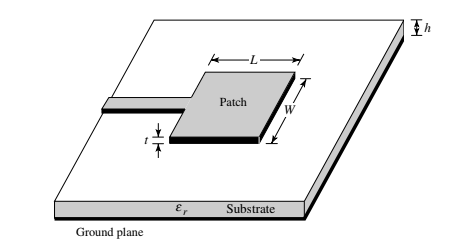
\includegraphics[width=1.0\textwidth]{figures/mspa_no_inset.png}
    \caption{Basic structure of a rectangular microstrip patch antenna (without inset feed).}
    \small Image adapted from \cite{balanis}.
    \label{fig:basic-mspa}
\end{figure}

\section{Feeding Techniques for Microstrip Patch Antennas}

There are several methods for feeding MSPAs, each with its own benefits and limitations:

\begin{itemize}
    \item \textbf{Microstrip Line Feed}: A simple and direct method, where a microstrip line is connected to the edge of the patch.
    \item \textbf{Inset Feed}: The microstrip line is inserted into the patch for impedance matching.
    \item \textbf{Coaxial Probe Feed}: A vertical coaxial probe connects the ground plane to the patch.
    \item \textbf{Aperture Coupled Feed}: Uses a slot in the ground plane to couple energy from a microstrip line below the substrate.
    \item \textbf{Proximity Coupled Feed}: Employs electromagnetic coupling between the feed line and the patch through overlapping substrates.
\end{itemize}

\subsection*{Inset Feeding}

Inset feeding is a modified microstrip line feed technique where the feed line is extended into the patch by a small distance, known as the \textit{inset distance}.

\begin{figure}[H]
    \centering
    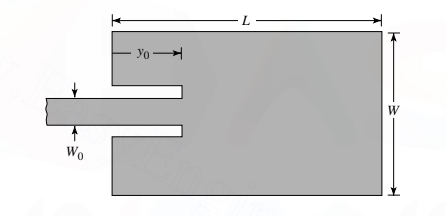
\includegraphics[width=1.0\textwidth]{figures/inset.png}
    \caption{Inset-fed rectangular microstrip patch antenna.}
    \small Image adapted from \cite{balanis}.
    \label{fig:inset-feed}
\end{figure}

\subsection*{Why Inset Feeding is Used}

The primary reason for inset feeding is to achieve \textbf{impedance matching} between the feed line (usually 50~$\Omega$) and the patch antenna, whose input impedance varies depending on the feed point location.

\begin{itemize}
    \item At the \textbf{edge of the patch}, the input impedance is high (typically 200–300~$\Omega$).
    \item By \textbf{moving the feed inward}, we reduce the input impedance to match the feed line.
    \item The \textbf{inset depth} is selected such that:
\end{itemize}

\[
Z_{\text{in}}(y_0) = Z_0 = 50~\Omega
\]

where $Z_{\text{in}}(y_0)$ is the input impedance at inset distance $y_0$, and $Z_0$ is the characteristic impedance of the microstrip line.

Inset feeding also helps maintain symmetry and reduces cross-polarization components, making it suitable for planar array applications.

\section*{Conclusion}

We have now understood the construction and operation of microstrip patch antennas, including detailed equations governing their geometry and resonance. Various feeding techniques were discussed, with inset feeding highlighted for impedance matching. This foundational knowledge will be used in the next chapter, where we simulate MSPAs under practical conditions with and without radome enclosures using ANSYS HFSS.

\chapter{Simulation Setup and Methodology}

This chapter details the simulation methodology adopted to evaluate the performance of a rectangular microstrip patch antenna (MSPA) under different conditions—specifically, in free space and enclosed within a flat radome. The antenna was designed for 6~GHz operation using an FR4 substrate, modeled and simulated using ANSYS HFSS. The methodology draws from standard antenna theory \cite{balanis} and radome design guidelines provided in \cite{swra705}.

\section{Design Specifications and Calculated Parameters}

The fundamental design inputs for the patch antenna are presented in Table~\ref{tab:designspecs}. These were used to calculate the required dimensions and parameters using standard MSPA design equations.

\begin{table}[htbp]
\centering
\caption{Patch Antenna Design Specifications}
\begin{tabular}{lc}
\toprule
\textbf{Parameter} & \textbf{Value} \\
\midrule
Operating frequency ($f_r$) & 6 GHz \\
Dielectric material & FR4 \\
Relative permittivity ($\varepsilon_r$) & 4.4 \\
Substrate thickness ($h$) & 1.6 mm \\
Loss tangent ($\tan \delta$) & 0.02 \\
\bottomrule
\end{tabular}
\label{tab:designspecs}
\end{table}

Using standard patch antenna equations, the calculated parameters are shown in Table~\ref{tab:calculatedvalues}:

\begin{table}[htbp]
\centering
\caption{Calculated Patch Antenna Parameters}
\begin{tabular}{lc}
\toprule
\textbf{Parameter} & \textbf{Value} \\
\midrule
Patch width ($W$) & 15.126 mm \\
Patch length ($L$) & 11.320 mm \\
Inset feed distance & 3.614 mm \\
Feed line width & 2.990 mm \\
Inset width & 4.600 mm \\
Inset depth & 3.800 mm \\
Effective permittivity ($\varepsilon_{\text{eff}}$) & 3.830 \\
Effective length ($L_{\text{eff}}$) & 12.774 mm \\
Fringing length ($\Delta L$) & 0.723 mm \\
Edge impedance & 284.13 $\Omega$ \\
\bottomrule
\end{tabular}
\label{tab:calculatedvalues}
\end{table}

\section{HFSS Simulation Workflow}

The antenna was modeled in ANSYS HFSS based on the above specifications using the following simulation steps:

\begin{itemize}
    \item Creation of the patch, ground plane, feed line, and substrate geometry.
    \item Assignment of FR4 as the substrate material with appropriate dielectric and loss properties.
    \item Application of waveports to excite the antenna.
    \item Radiation boundary setup to mimic free-space conditions.
    \item Mesh refinement using adaptive meshing for improved solution accuracy.
    \item Solution sweep over frequency range to obtain $S_{11}$ and gain plots.
\end{itemize}

\section{Flat Radome Design and Placement}

A flat radome was introduced to study its influence on antenna characteristics. The radome was modeled as a planar dielectric cover and designed using optimal thickness expressions provided in \cite{swra705}:

\begin{equation}
t_{\text{optimum}} = n \cdot \frac{\lambda_0}{2 \sqrt{\varepsilon_r}},
\end{equation}

where:
\begin{itemize}
    \item $n$ is a positive integer,
    \item $\lambda_0$ is the free-space wavelength,
    \item $\varepsilon_r$ is the radome material's relative permittivity.
\end{itemize}

The radome was placed at a specific spacing from the antenna to minimize reflections and multipath effects. This optimal separation is given by:

\begin{equation}
D_{\text{opt}} = n \cdot \frac{\lambda_0}{2}
\end{equation}

\begin{figure}[H]
\centering
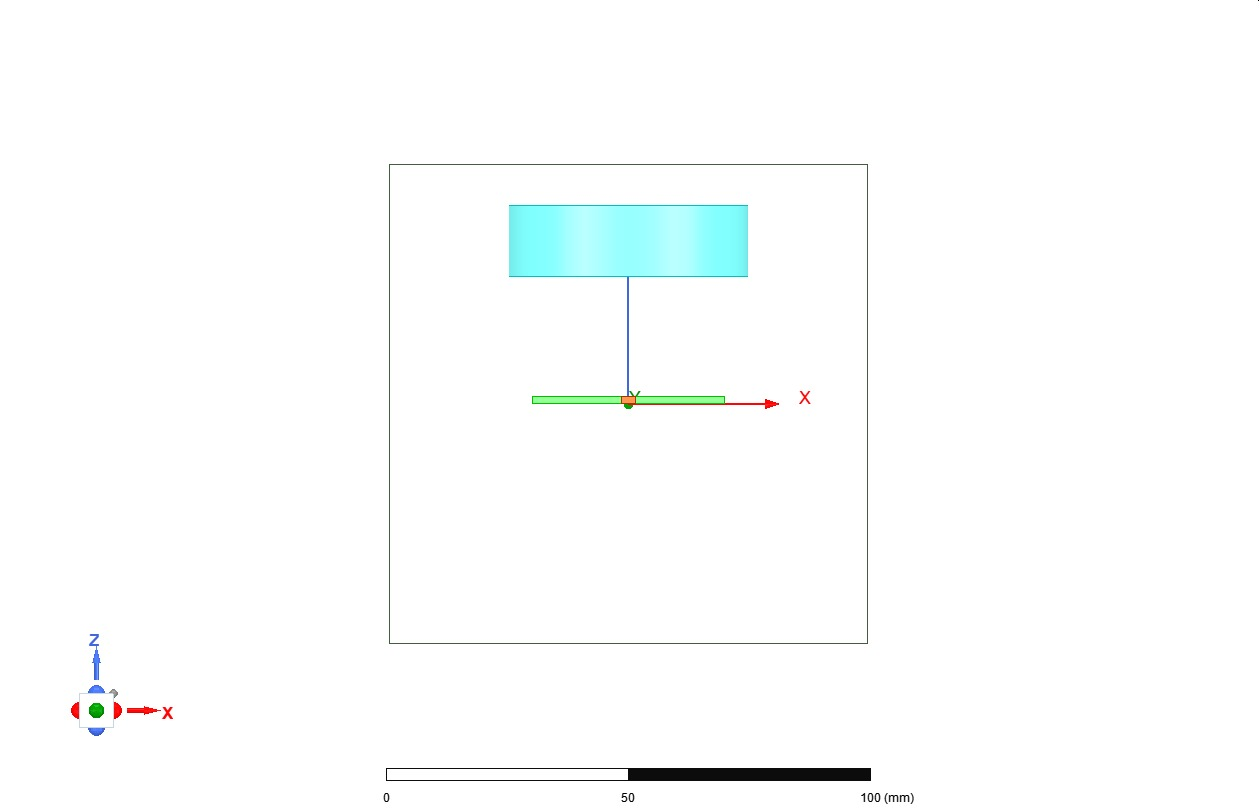
\includegraphics[width=0.8\textwidth]{figures/flat_radome.jpeg}
\caption{Front view of the simulation setup showing the patch antenna enclosed within a flat PMMA radome in ANSYS HFSS.}
\label{fig:flat_radome}
\end{figure}

\subsection*{Radome Material Selection}

In this study, the flat radome was modeled using PMMA (Plexiglass), which is commonly used for RF enclosures due to its mechanical strength and RF transparency. The material parameters used in ANSYS HFSS are listed in Table~\ref{tab:pmma-properties}.

\begin{table}[H]
\centering
\caption{Material Properties of PMMA Used in Simulation}
\begin{tabular}{lcl}
\toprule
\textbf{Parameter} & \textbf{Value} & \textbf{Units} \\
\midrule
Relative permittivity ($\varepsilon_r$) & 2.8 & -- \\
Relative permeability ($\mu_r$) & 1 & -- \\
Dielectric loss tangent ($\tan\delta$) & 0.001 & -- \\
Bulk conductivity & $1 \times 10^{-16}$ & S/m \\
Mass density & 1180 & kg/m$^3$ \\
Measured frequency & 6 GHz & Hz \\
\bottomrule
\end{tabular}
\label{tab:pmma-properties}
\end{table}

\section{Simulation Campaign}

The following simulation cases were conducted in ANSYS HFSS:

\begin{enumerate}
    \item Patch antenna in free space (baseline)
    \item Patch antenna enclosed by a flat PMMA radome
\end{enumerate}

In each case, key performance metrics were extracted, including return loss ($S_{11}$), VSWR, gain patterns, and 3D radiation plots. These results are analyzed and compared in the following chapter.

\section{Outlook for Future Work}

While this study primarily focused on evaluating the influence of flat radomes, several future directions can enhance the simulation methodology:

\begin{itemize}
    \item \textbf{Design Optimization:} Use of metaheuristic algorithms (e.g., genetic algorithms, PSO) to optimize patch dimensions and radome thickness.
    \item \textbf{Advanced Substrates:} Exploration of low-loss substrates like Rogers RT/duroid series for high-performance designs.
    \item \textbf{Environmental Effects:} Study of temperature and humidity influence on dielectric properties and antenna performance.
    \item \textbf{Multi-layer Radomes:} Evaluation of layered dielectric structures for enhanced frequency selectivity and mechanical robustness.
\end{itemize}

These extensions would strengthen the practical applicability of the proposed antenna system, particularly for radio astronomy or high-frequency communication applications.

\section*{Conclusion}

This chapter described the complete simulation pipeline—from calculating patch dimensions to radome modeling in HFSS. The flat PMMA radome was modeled using realistic material parameters, and the simulation configurations were designed to compare the antenna’s free-space performance with radome-enclosed behavior. In the next chapter, we present and interpret the results of these simulations, analyzing key metrics like return loss, gain, and radiation pattern.

\chapter{Results}

This chapter presents the simulation results of the patch antenna under three scenarios:
\begin{itemize}
    \item Baseline without radome
    \item Parametric sweep of patch antenna parameters
    \item With a flat radome
\end{itemize}
Key performance indicators such as return loss, VSWR, gain, directivity, and radiation patterns are analyzed.

\section{Performance Without Radome}

\subsection{Return Loss and VSWR}

\begin{figure}[H]
    \centering
    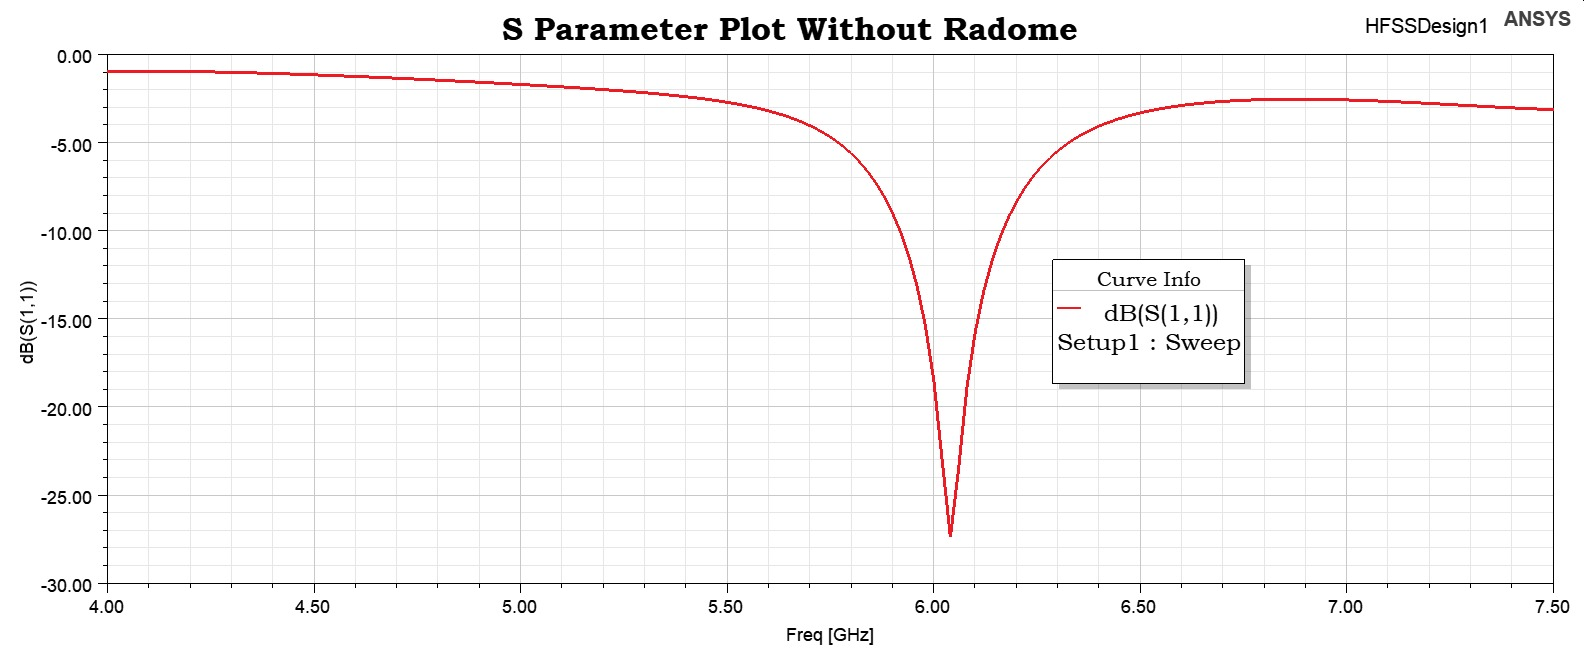
\includegraphics[width=1.0\textwidth]{figures/without_radome/s11.jpeg}
    \caption{Simulated S11 (return loss) of the patch antenna without radome.}
    \label{fig:res-without-s11}
\end{figure}

Figure~\ref{fig:res-without-s11} illustrates the return loss (S11) performance of the patch antenna in free space. The deep notch around the center frequency (approximately 6 GHz) indicates efficient impedance matching, as values below $-10$ dB suggest minimal reflection. The sharper and deeper the dip, the better the resonance quality.

\begin{figure}[H]
    \centering
    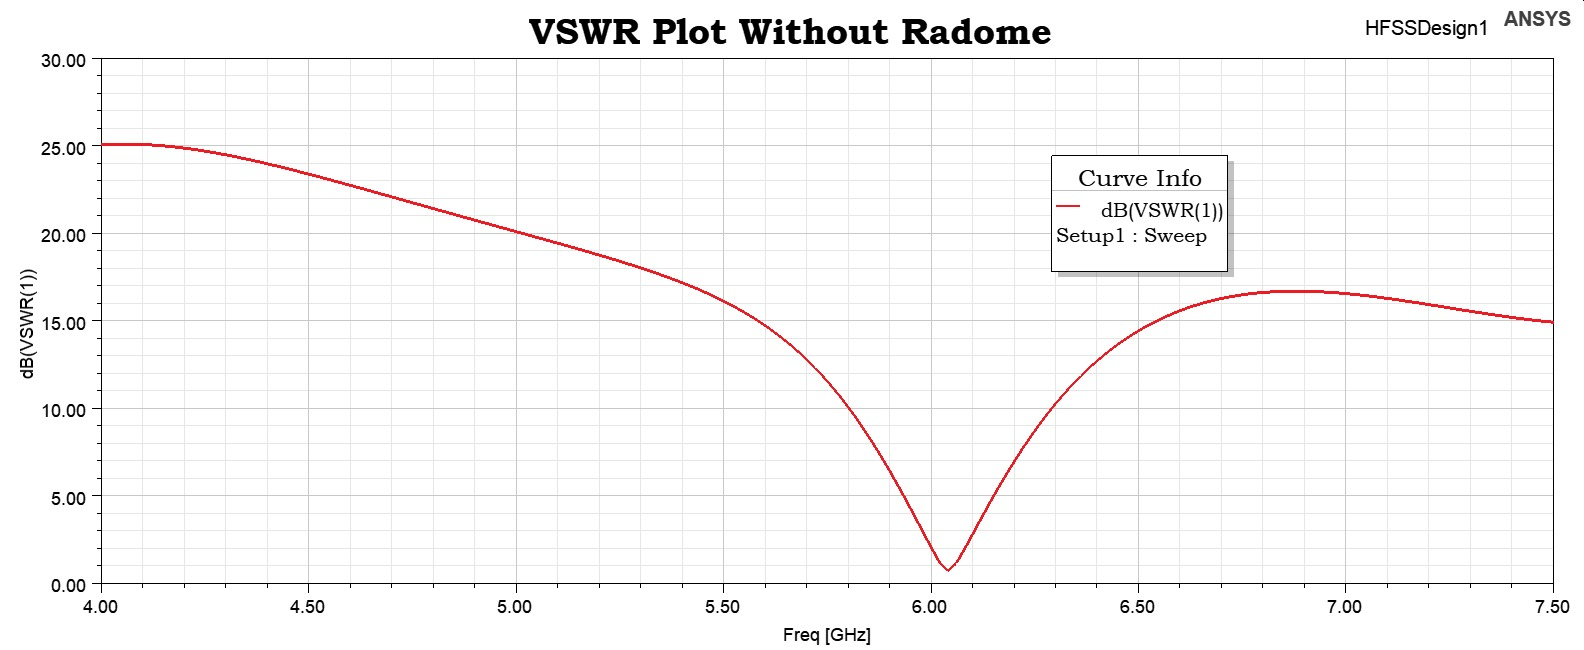
\includegraphics[width=1.0\textwidth]{figures/without_radome/VSWR.jpeg}
    \caption{Simulated VSWR of the patch antenna without radome.}
    \label{fig:res-without-vswr}
\end{figure}

The VSWR plot in Figure~\ref{fig:res-without-vswr} shows a corresponding dip near 6 GHz. A VSWR close to 1 indicates ideal matching, and values below 2 are generally acceptable. The shape and location of the curve match the S11 data, further validating the antenna's tuning.

\subsection{Gain Characteristics}

\begin{figure}[H]
    \centering
    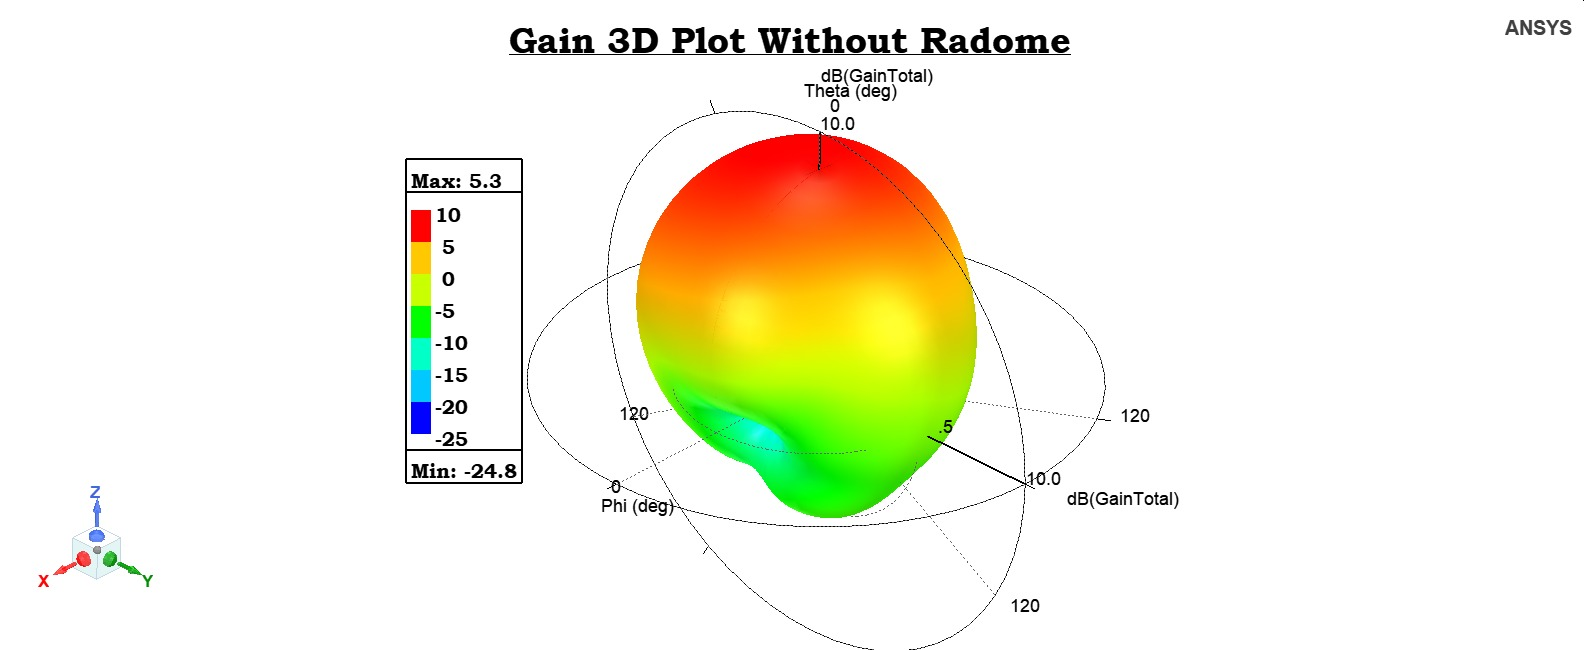
\includegraphics[width=1.0\textwidth]{figures/without_radome/gain plot.jpeg}
    \caption{Simulated gain of the patch antenna without radome.}
    \label{fig:res-without-gain}
\end{figure}

Figure~\ref{fig:res-without-gain} presents the frequency response of gain. The gain peaks near resonance and gradually falls off toward the band edges, a typical trend in patch antennas. This result reflects good radiation efficiency with a directional pattern. The gain level is suitable for point-to-point or sector-based wireless communication applications.

\begin{figure}[H]
    \centering
    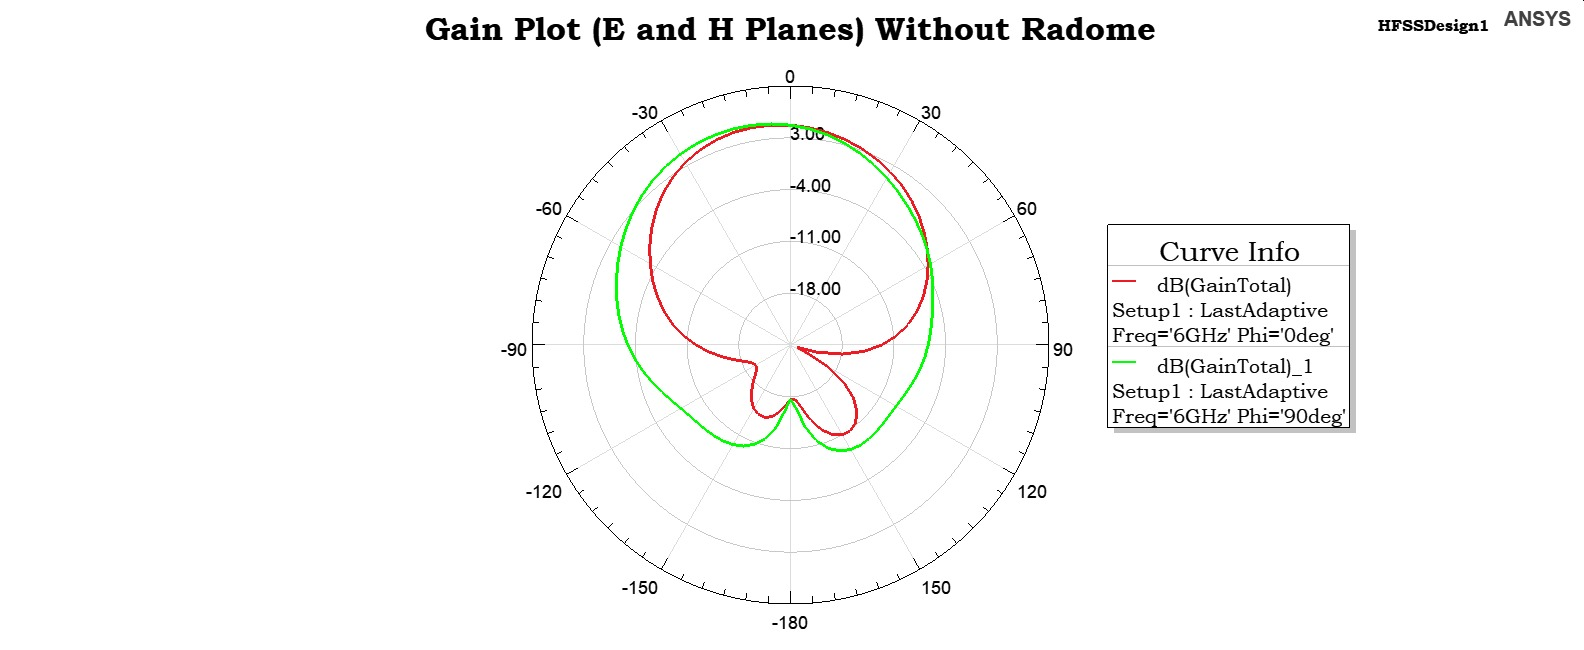
\includegraphics[width=1.0\textwidth]{figures/without_radome/Gain.jpeg}
    \caption{Gain pattern of the patch antenna without radome in both E-plane and H-plane.}
    \label{fig:res-gain-ehplane}
\end{figure}

Figure~\ref{fig:res-gain-ehplane} presents the 2D radiation patterns in the principal planes. The E-plane (elevation cut) shows the variation of gain with respect to vertical angle, while the H-plane (azimuthal cut) illustrates gain variation in the horizontal plane. The patterns confirm the directional behavior of the antenna and reveal its symmetry and front-to-back ratio. The close alignment of the main lobes in both planes suggests well-controlled beam shaping.

\subsection{Additional \texorpdfstring{$rE$}{rE} Overview}

\begin{figure}[H]
    \centering
    \includegraphics[width=1.0\textwidth]{figures/without_radome/co.jpeg}
    \caption{Co-polarization response of the patch antenna without radome.}
    \label{fig:res-co}
\end{figure}

\begin{figure}[H]
    \centering
    \includegraphics[width=1.0\textwidth]{figures/without_radome/cross.jpeg}
    \caption{Cross-polarization response of the patch antenna without radome.}
    \label{fig:res-cross}
\end{figure}

Figures~\ref{fig:res-co} and \ref{fig:res-cross} illustrate the co-polarization and cross-polarization responses of the patch antenna in the absence of a radome. The co-polarized field represents the desired polarization component aligned with the antenna's radiating axis, while the cross-polarized field indicates orthogonal components that are typically unwanted.

The co-polarization plot shows a strong, well-defined main lobe centered around the boresight, confirming that the antenna radiates efficiently in the intended polarization. In contrast, the cross-polarization level remains significantly lower across all angles, indicating minimal polarization leakage and strong polarization purity—an important factor in communication systems that rely on polarization isolation.

\begin{figure}[H]
    \centering
    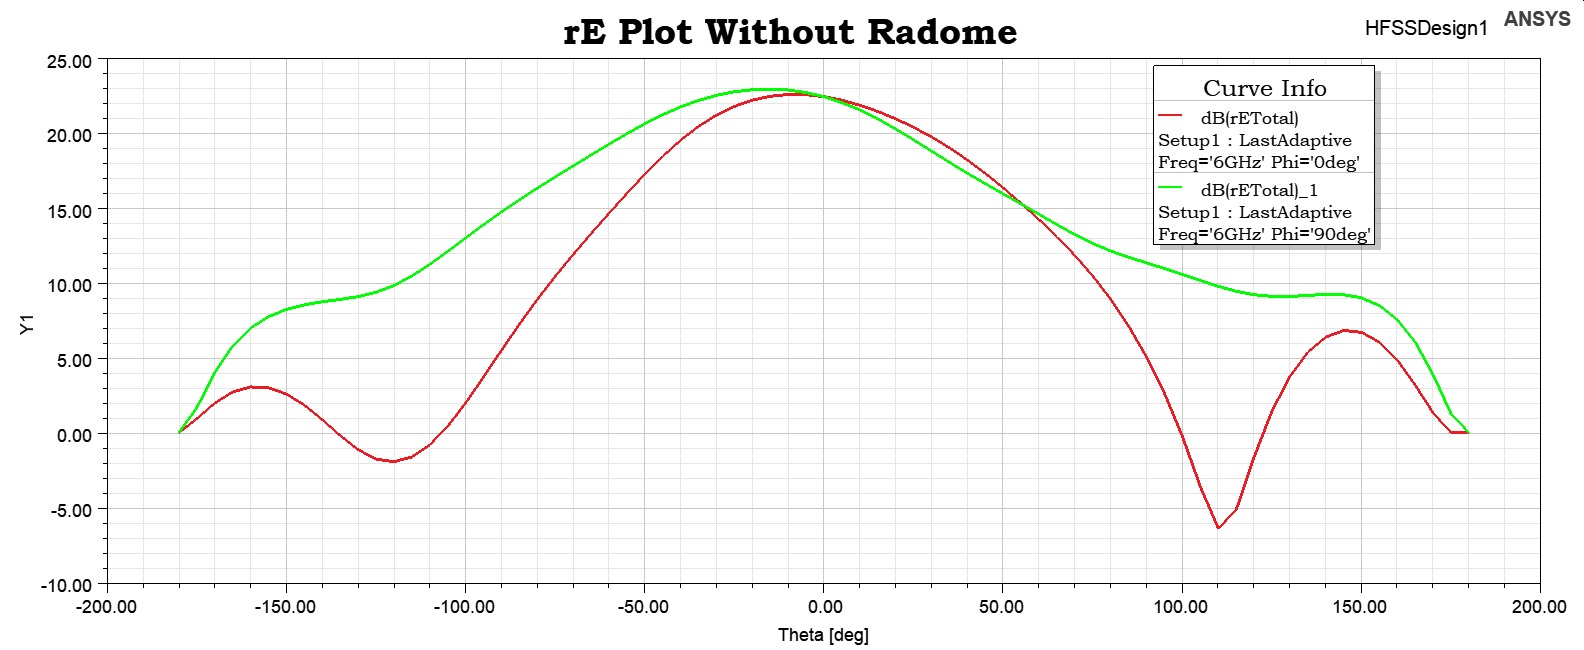
\includegraphics[width=1.0\textwidth]{figures/without_radome/rE.jpeg}
    \caption{General $rE$ field distribution without radome.}
    \label{fig:res-flat-re-overview}
\end{figure}

Figure~\ref{fig:res-flat-re-overview} shows the normalized electric field distribution ($rE$) in the far field. The pattern is symmetric and exhibits a broadside radiation characteristic, with energy concentrated normal to the patch surface. The absence of asymmetries or spurious sidelobes further confirms that the antenna operates as intended without distortions caused by external structures such as radomes.

\subsection{Parametric Sweep of Inset Feed}

\begin{figure}[H]
    \centering
    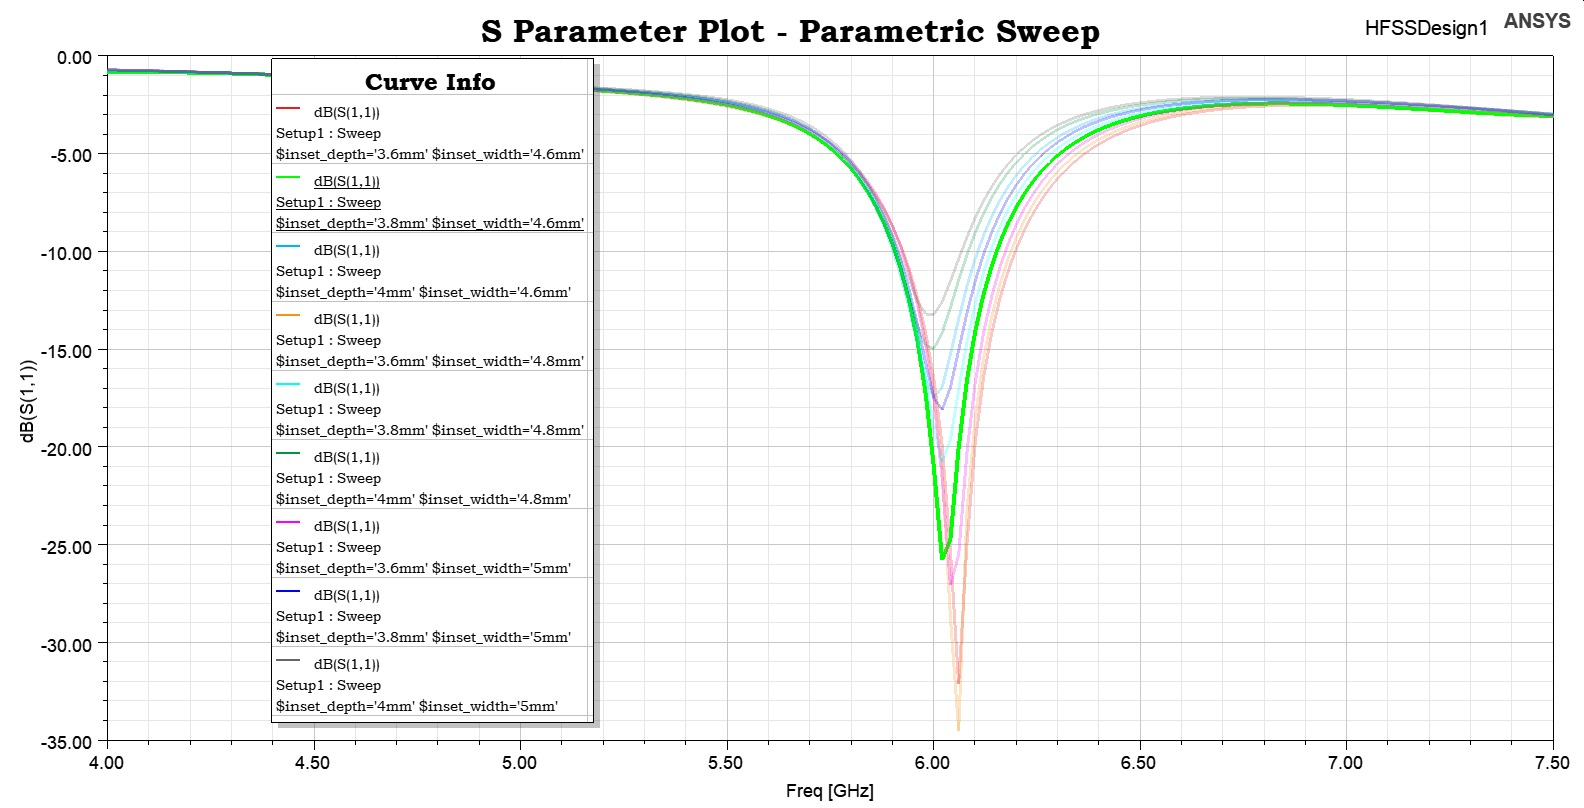
\includegraphics[width=1.0\textwidth]{figures/parametric_sweep/best parameter.jpeg}
    \caption{Identified optimal inset feed parameters from the parametric sweep.}
    \label{fig:res-param-best}
\end{figure}

Figure~\ref{fig:res-param-best} summarizes the optimal inset feed location and width for achieving best impedance match. Proper tuning of these parameters is critical for maximum power transfer and is reflected in a lower S11 and better VSWR.

\begin{figure}[H]
    \centering
    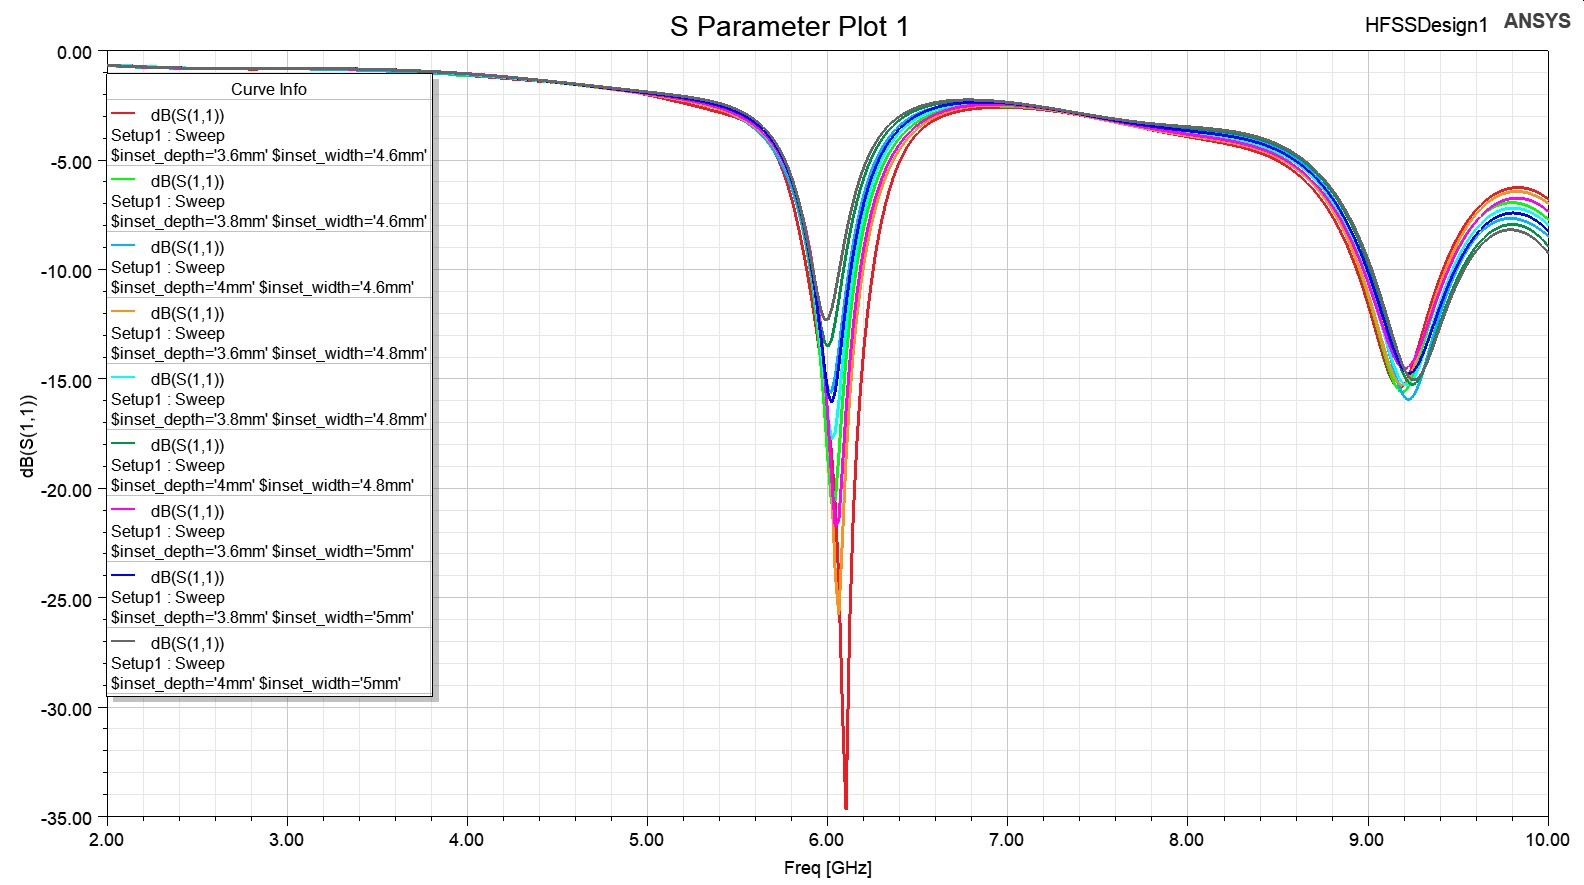
\includegraphics[width=1.0\textwidth]{figures/parametric_sweep/parametric analysis.jpeg}
    \caption{General overview of the parametric analysis for feed inset optimization.}
    \label{fig:res-param-analysis}
\end{figure}

Figure~\ref{fig:res-param-analysis} demonstrates the effect of varying feed positions on return loss. The ideal combination is the one that yields the deepest notch around the target frequency. This iterative approach provides insights into the physical sensitivity of the antenna to feed location.

\noindent
Note: The same feed dimensions will be reused for radome studies.

% -------------------------------------------------------------------

\section{Performance with Flat Radome}

\subsection{Parametric Sweep of Inter-Radome Distance}

\begin{figure}[H]
    \centering
    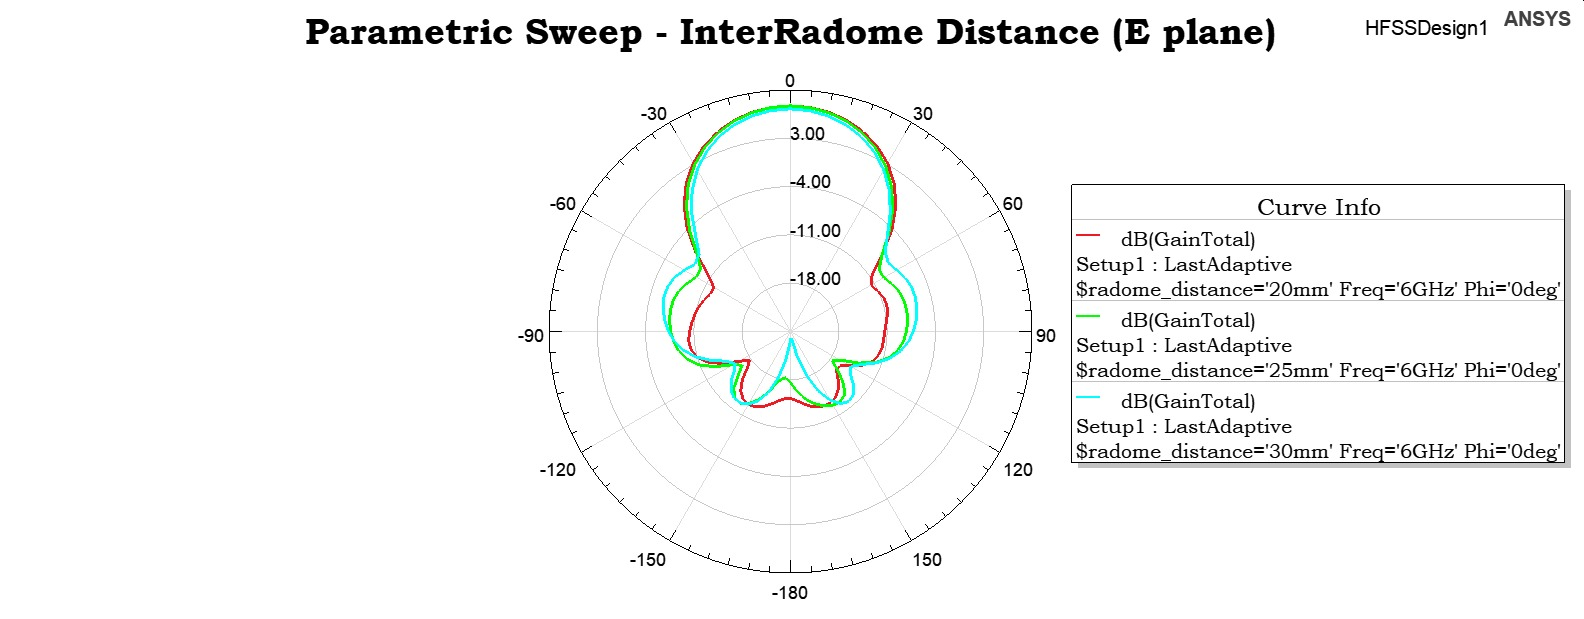
\includegraphics[width=1.0\textwidth]{figures/parametric_sweep/Radome distance (E plane).jpeg}
    \caption{Gain variation in the E-plane for different inter-radome (airgap) distances.}
    \label{fig:res-gap-gain-eplane}
\end{figure}

\begin{figure}[H]
    \centering
    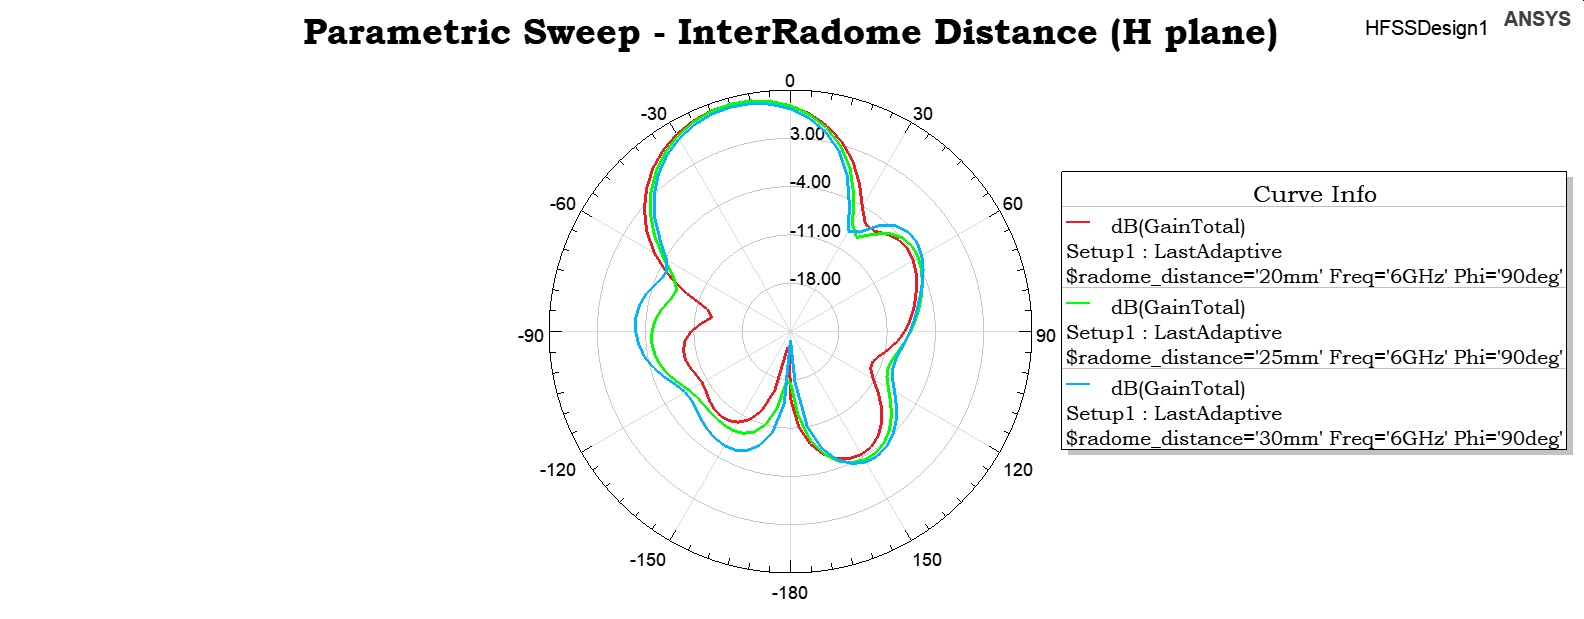
\includegraphics[width=1.0\textwidth]{figures/parametric_sweep/radome distance (H plane).jpeg}
    \caption{Gain variation in the H-plane for different inter-radome (airgap) distances.}
    \label{fig:res-gap-gain-hplane}
\end{figure}

Figures~\ref{fig:res-gap-gain-eplane} and \ref{fig:res-gap-gain-hplane} show how the gain pattern evolves in the E-plane and H-plane respectively as the distance between the antenna and the radome changes. Both plots highlight the existence of an optimal separation where gain is maximized due to constructive field interaction.

Deviating from this optimal point leads to degraded gain, caused by near-field phase mismatch and partial destructive interference. This reinforces the importance of careful mechanical design and spacing in practical antenna–radome integration.

\subsection{Gain Characteristics with Radome}

\begin{figure}[H]
    \centering
    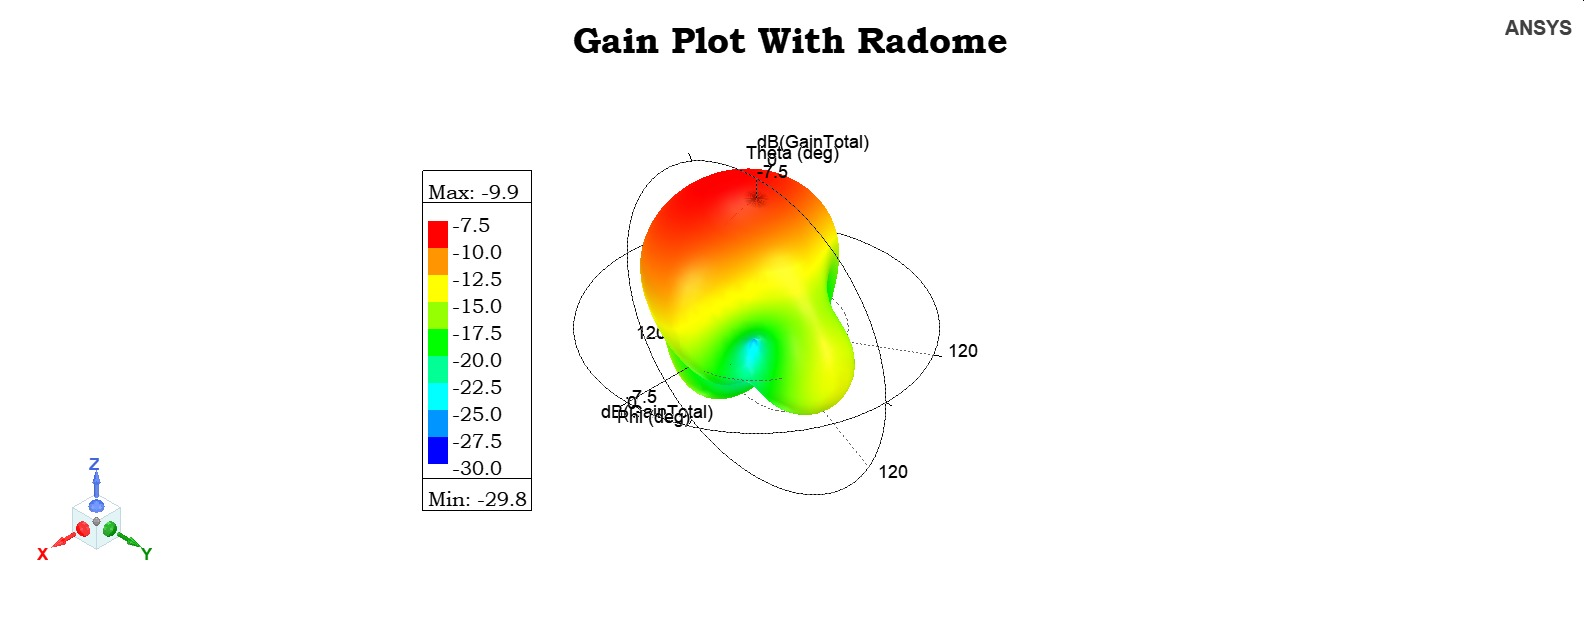
\includegraphics[width=1.0\textwidth]{figures/with_radome/gain plot.jpeg}
    \caption{Simulated gain of the patch antenna with flat radome.}
    \label{fig:res-with-gain-radome}
\end{figure}

Figure~\ref{fig:res-with-gain-radome} shows the gain response of the patch antenna when enclosed within a flat radome. While the overall shape of the curve remains similar to the no-radome case, a slight reduction in peak gain is observed, particularly near the resonant frequency. This reduction is attributed to dielectric loading and partial reflection losses introduced by the radome material. Despite this, the antenna still maintains a directional radiation pattern with adequate gain for practical deployment, indicating that the radome's impact on gain is minimal.

\subsection{Return Loss and VSWR}

\begin{figure}[H]
    \centering
    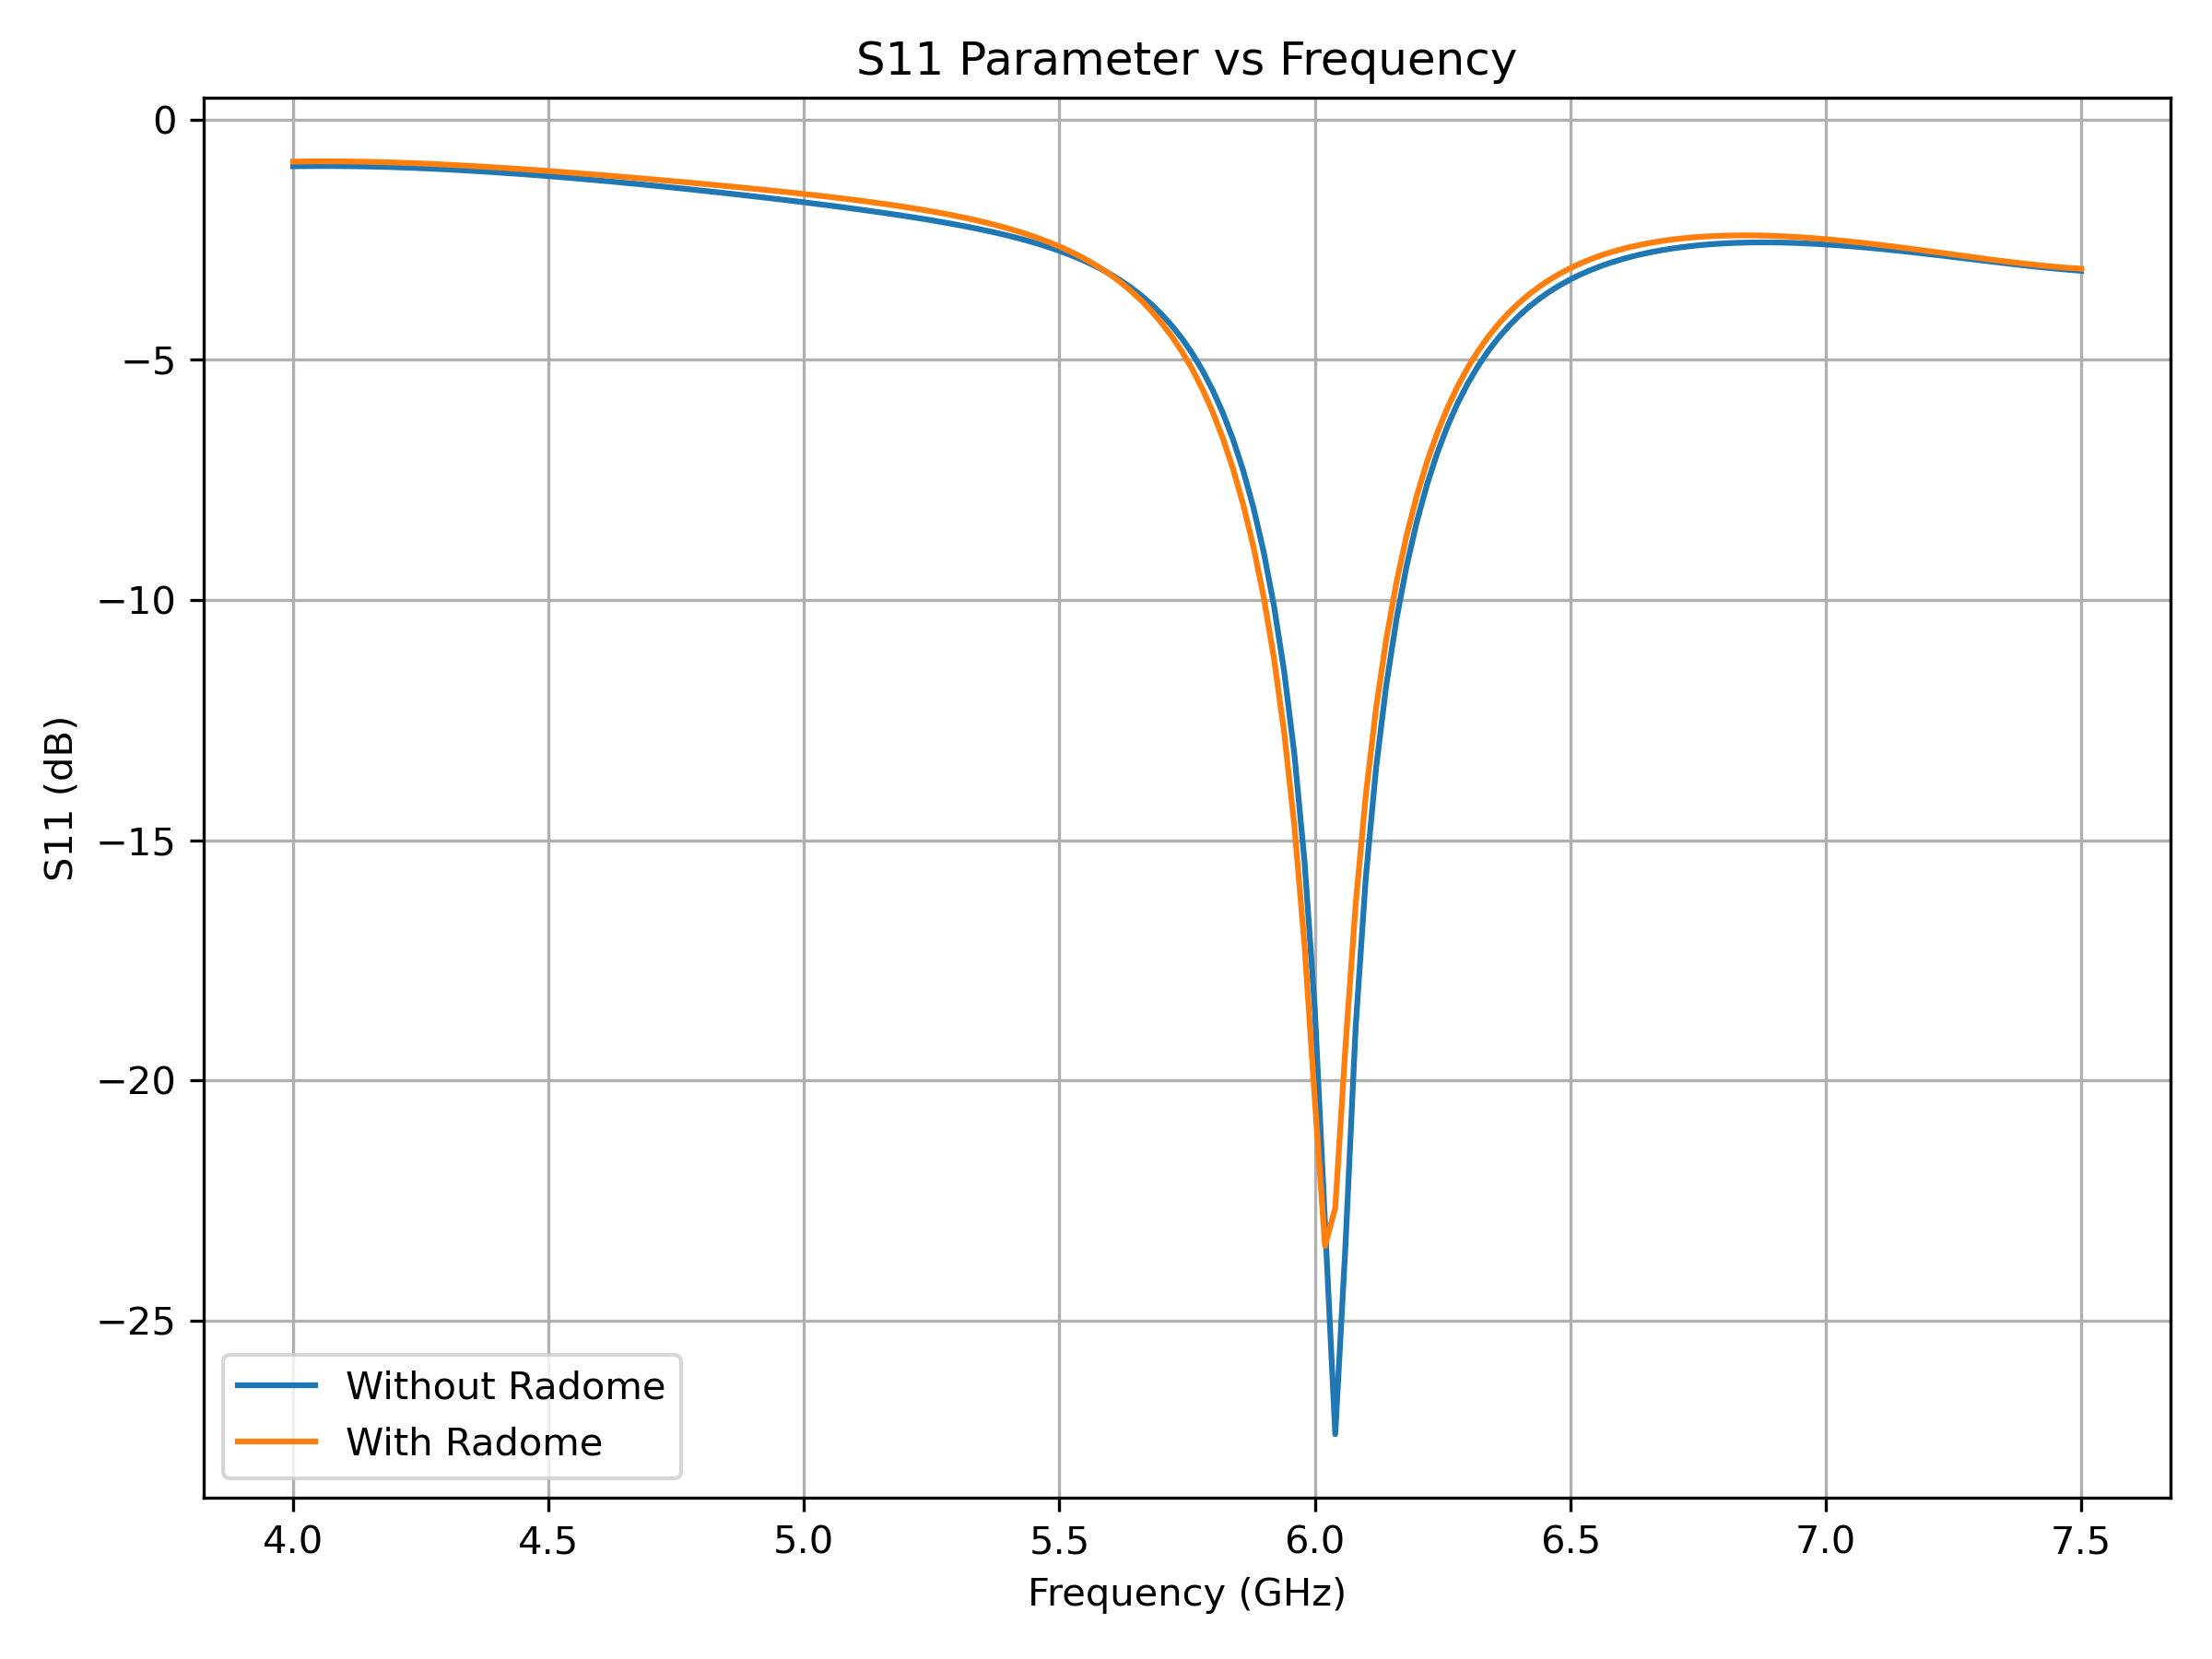
\includegraphics[width=1.0\textwidth]{figures/comparison_flat_radome/s11.png}
    \caption{Simulated S11 of the patch antenna with flat radome.}
    \label{fig:res-flat-s11}
\end{figure}

Figure~\ref{fig:res-flat-s11} depicts a noticeable shift in the return loss curve due to the introduction of the PMMA radome. The frequency shift indicates a slight detuning effect caused by the dielectric loading. The dip is slightly shallower, suggesting marginal impedance mismatch introduced by the radome material.

\begin{figure}[H]
    \centering
    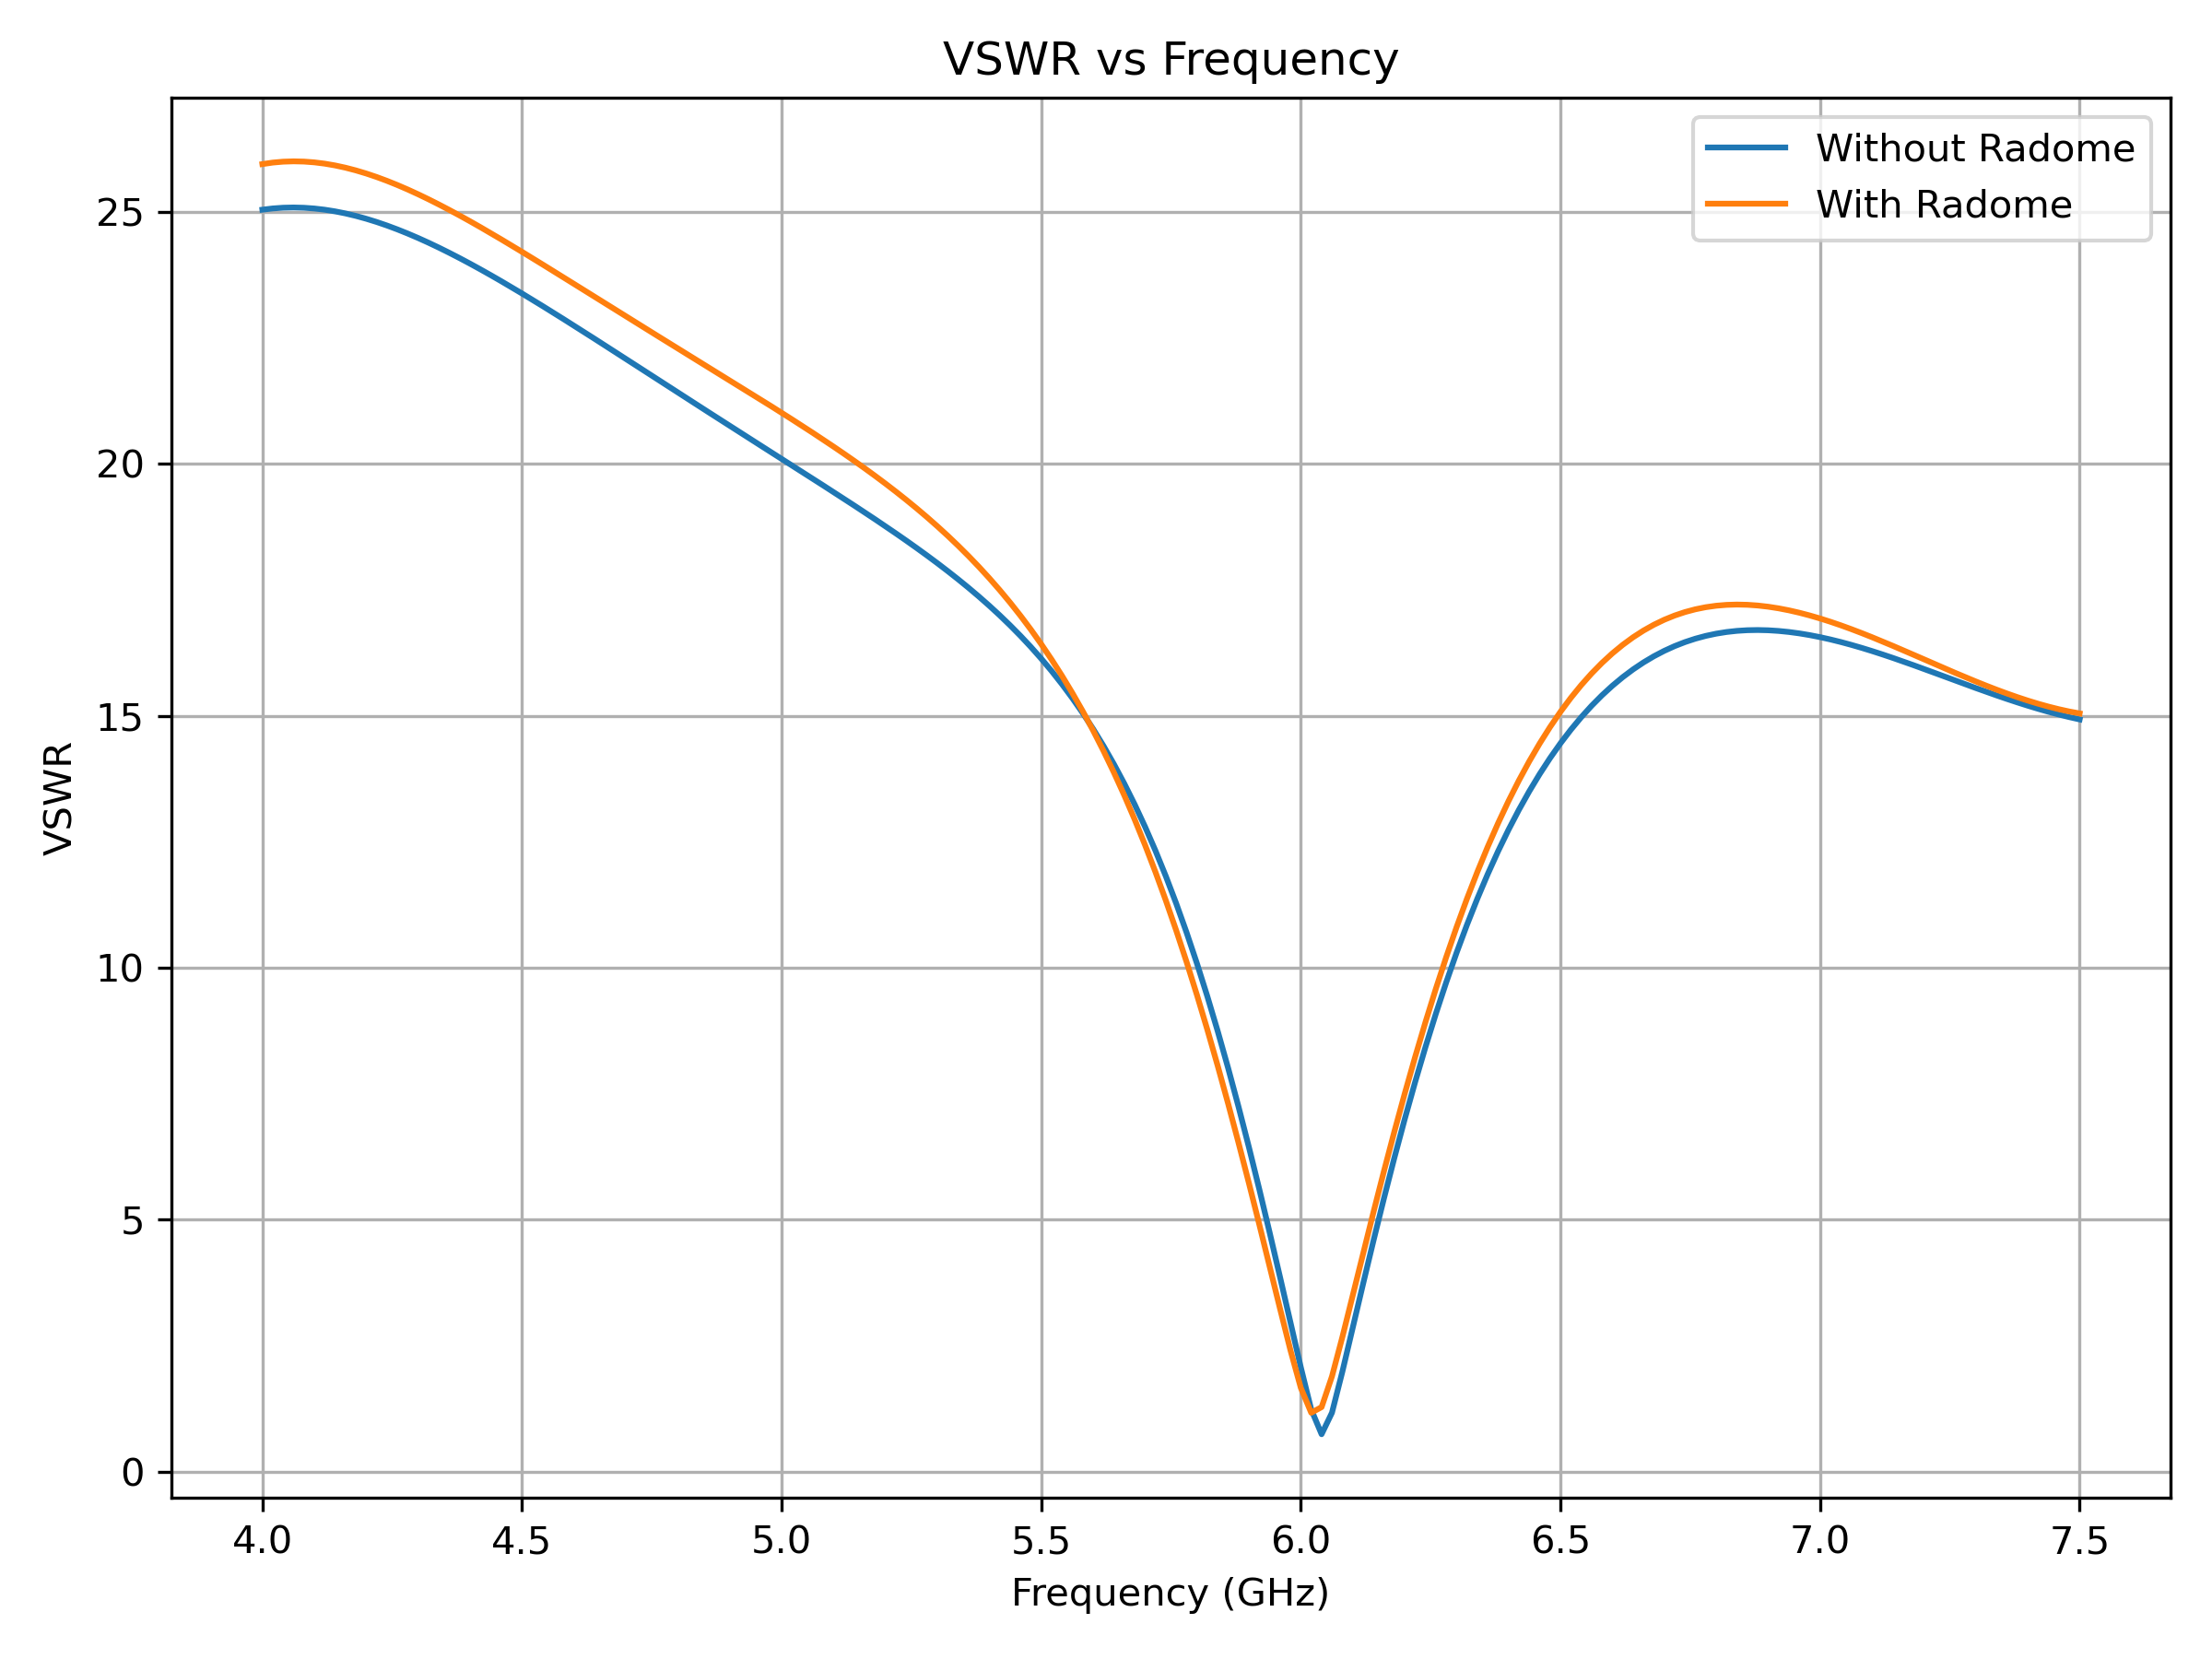
\includegraphics[width=1.0\textwidth]{figures/comparison_flat_radome/vswr.png}
    \caption{Simulated VSWR of the patch antenna with flat radome.}
    \label{fig:res-flat-vswr}
\end{figure}

In Figure~\ref{fig:res-flat-vswr}, the VSWR is slightly higher than the baseline case, reinforcing the return loss trend. Although still under 2, indicating acceptable performance, the result confirms that the radome introduces a small impedance mismatch.

\subsection{Gain across Frequencies (E-Plane)}

The E-plane gain patterns (phi=0°) show the antenna's performance with and without a radome at various frequencies.

\begin{figure}[H]
\centering
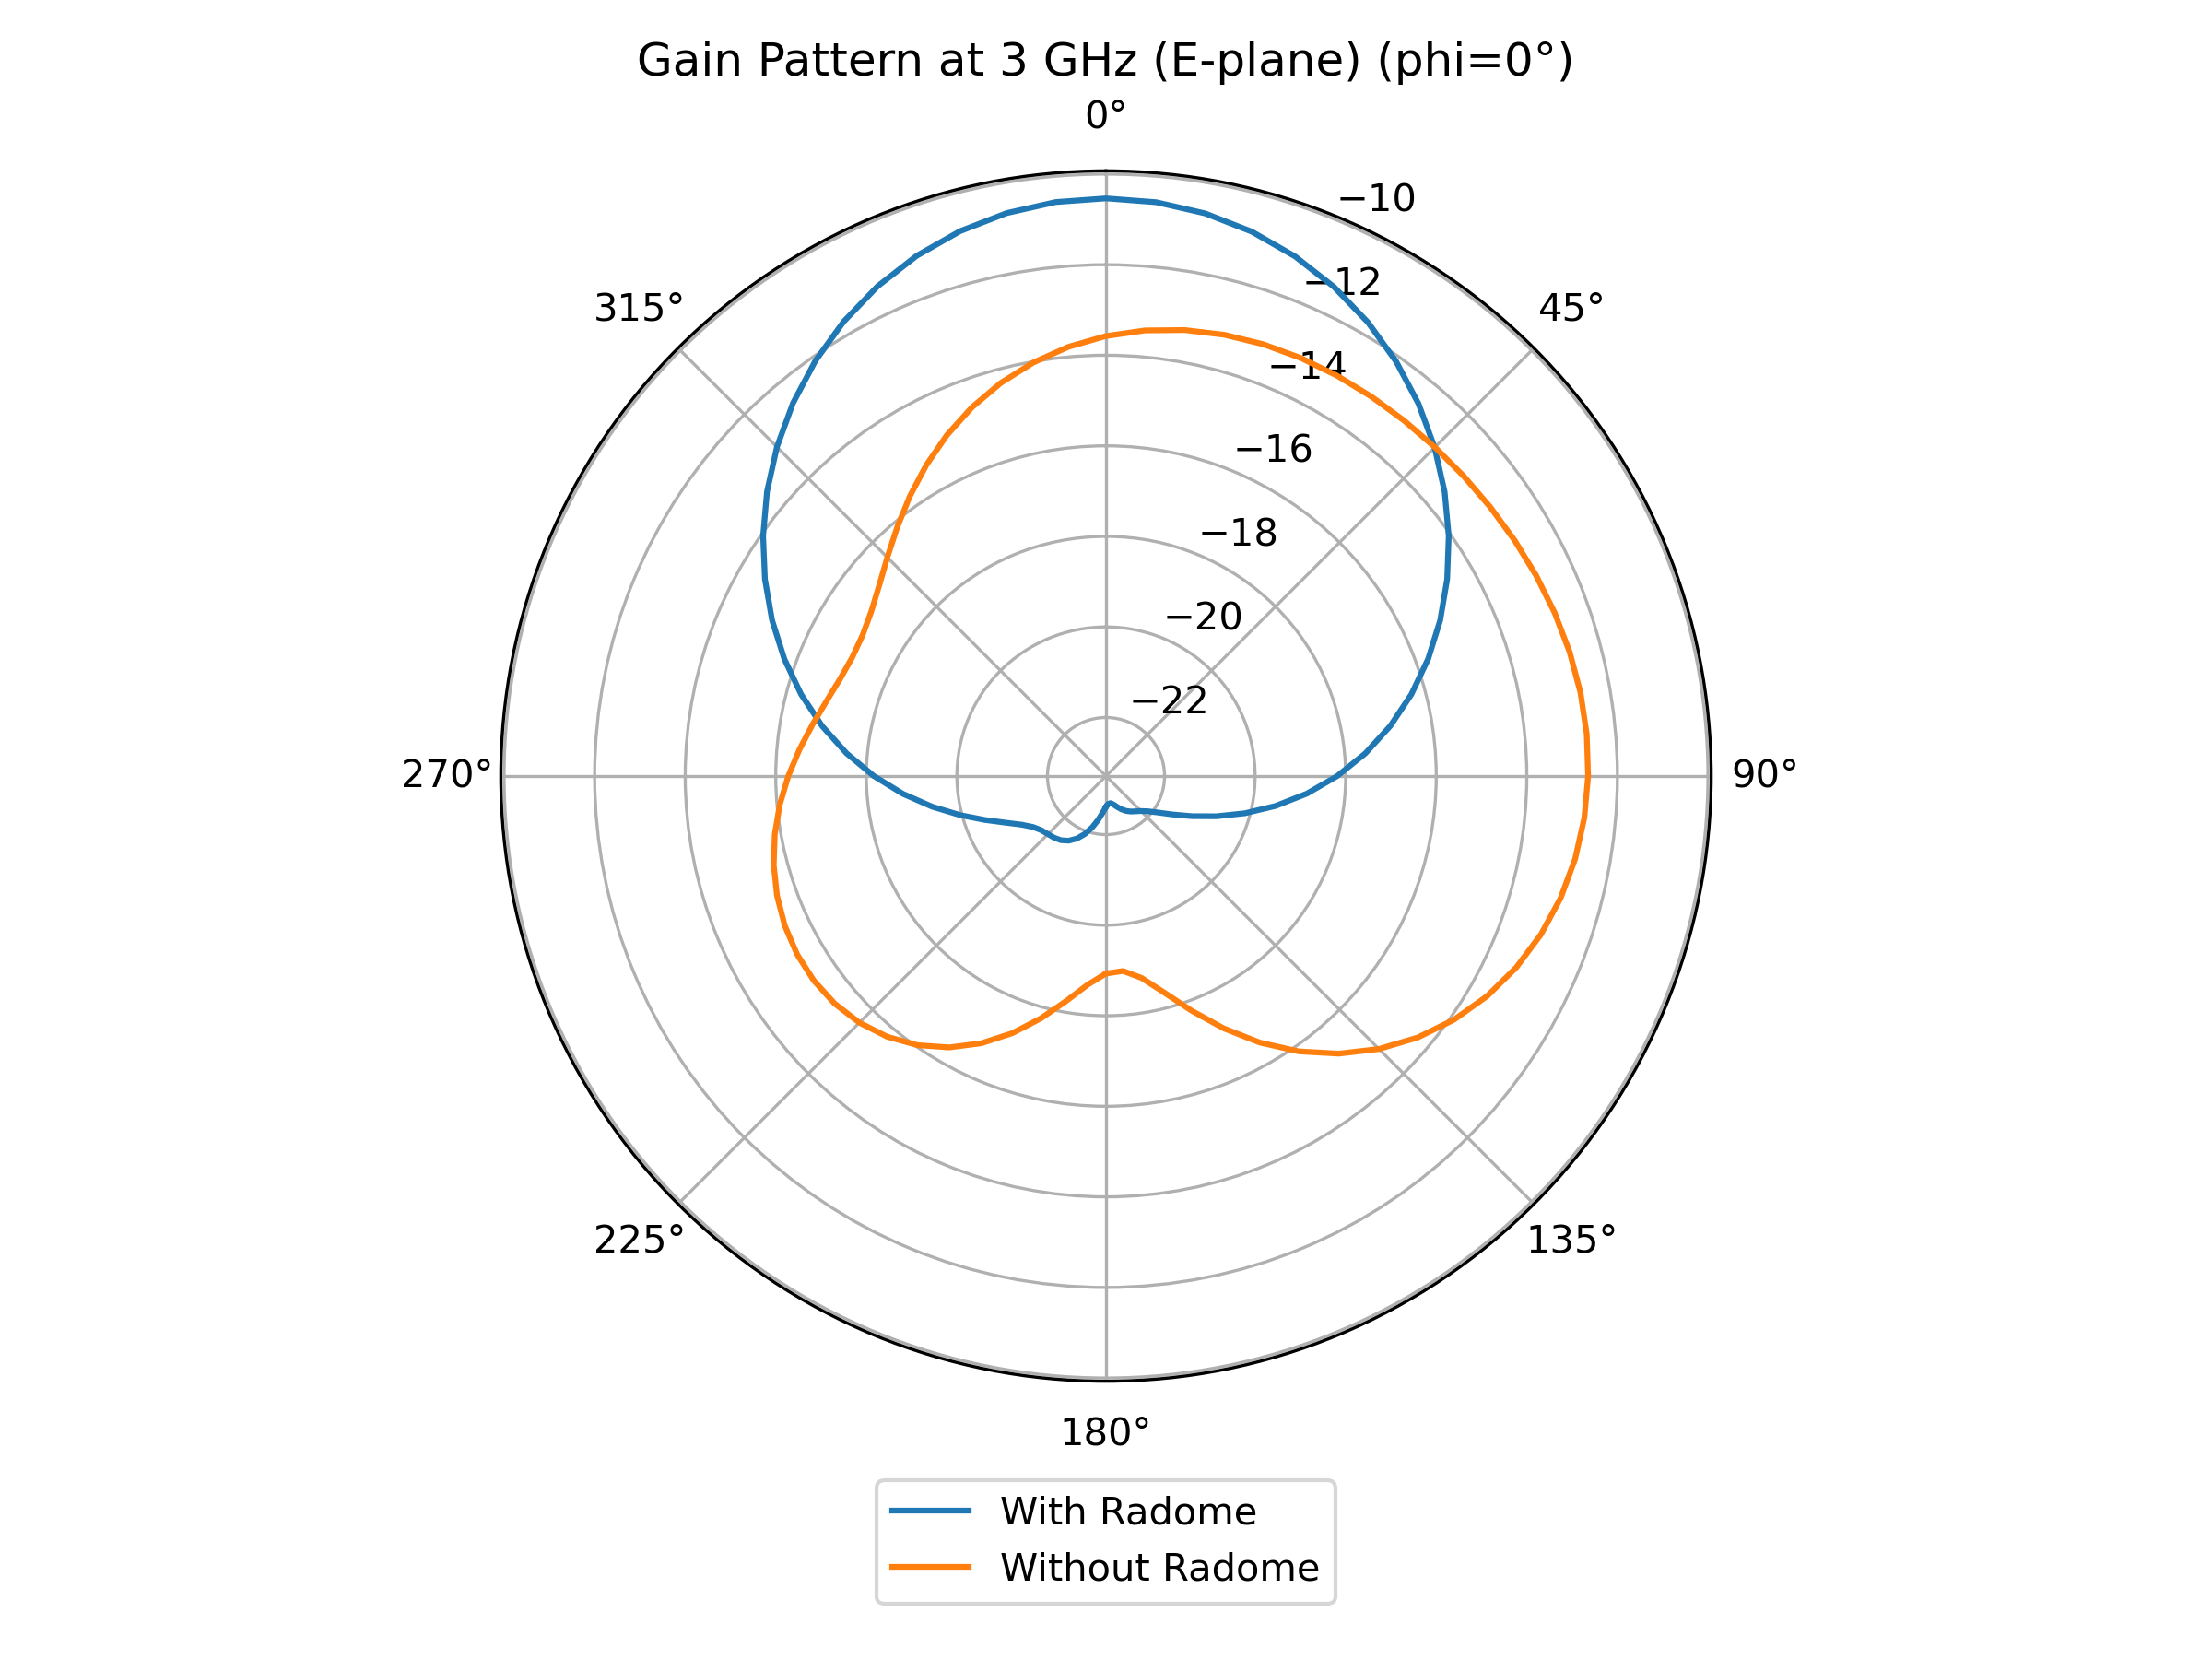
\includegraphics[width=1.0\textwidth]{figures/comparison_flat_radome/gainE_3_GHz.png}
\caption{Simulated gain of the patch antenna with flat radome at 3,GHz.}
\label{fig:res-flat-gainE3}
\end{figure}

Figure~\ref{fig:res-flat-gainE3} illustrates the radiation performance at the lower edge of the band (3 GHz) in the E-plane. Here, the gain of the antenna with the flat radome (blue line) is noticeably reduced compared to the free-space performance (orange line), particularly in the main lobe. The maximum gain without the radome is around -12 dB, while with the radome, it increases to approximately -10 dB. This suggests increased reflection and possible absorption by the radome at this off-resonant frequency, leading to a degradation in performance.

\begin{figure}[H]
\centering
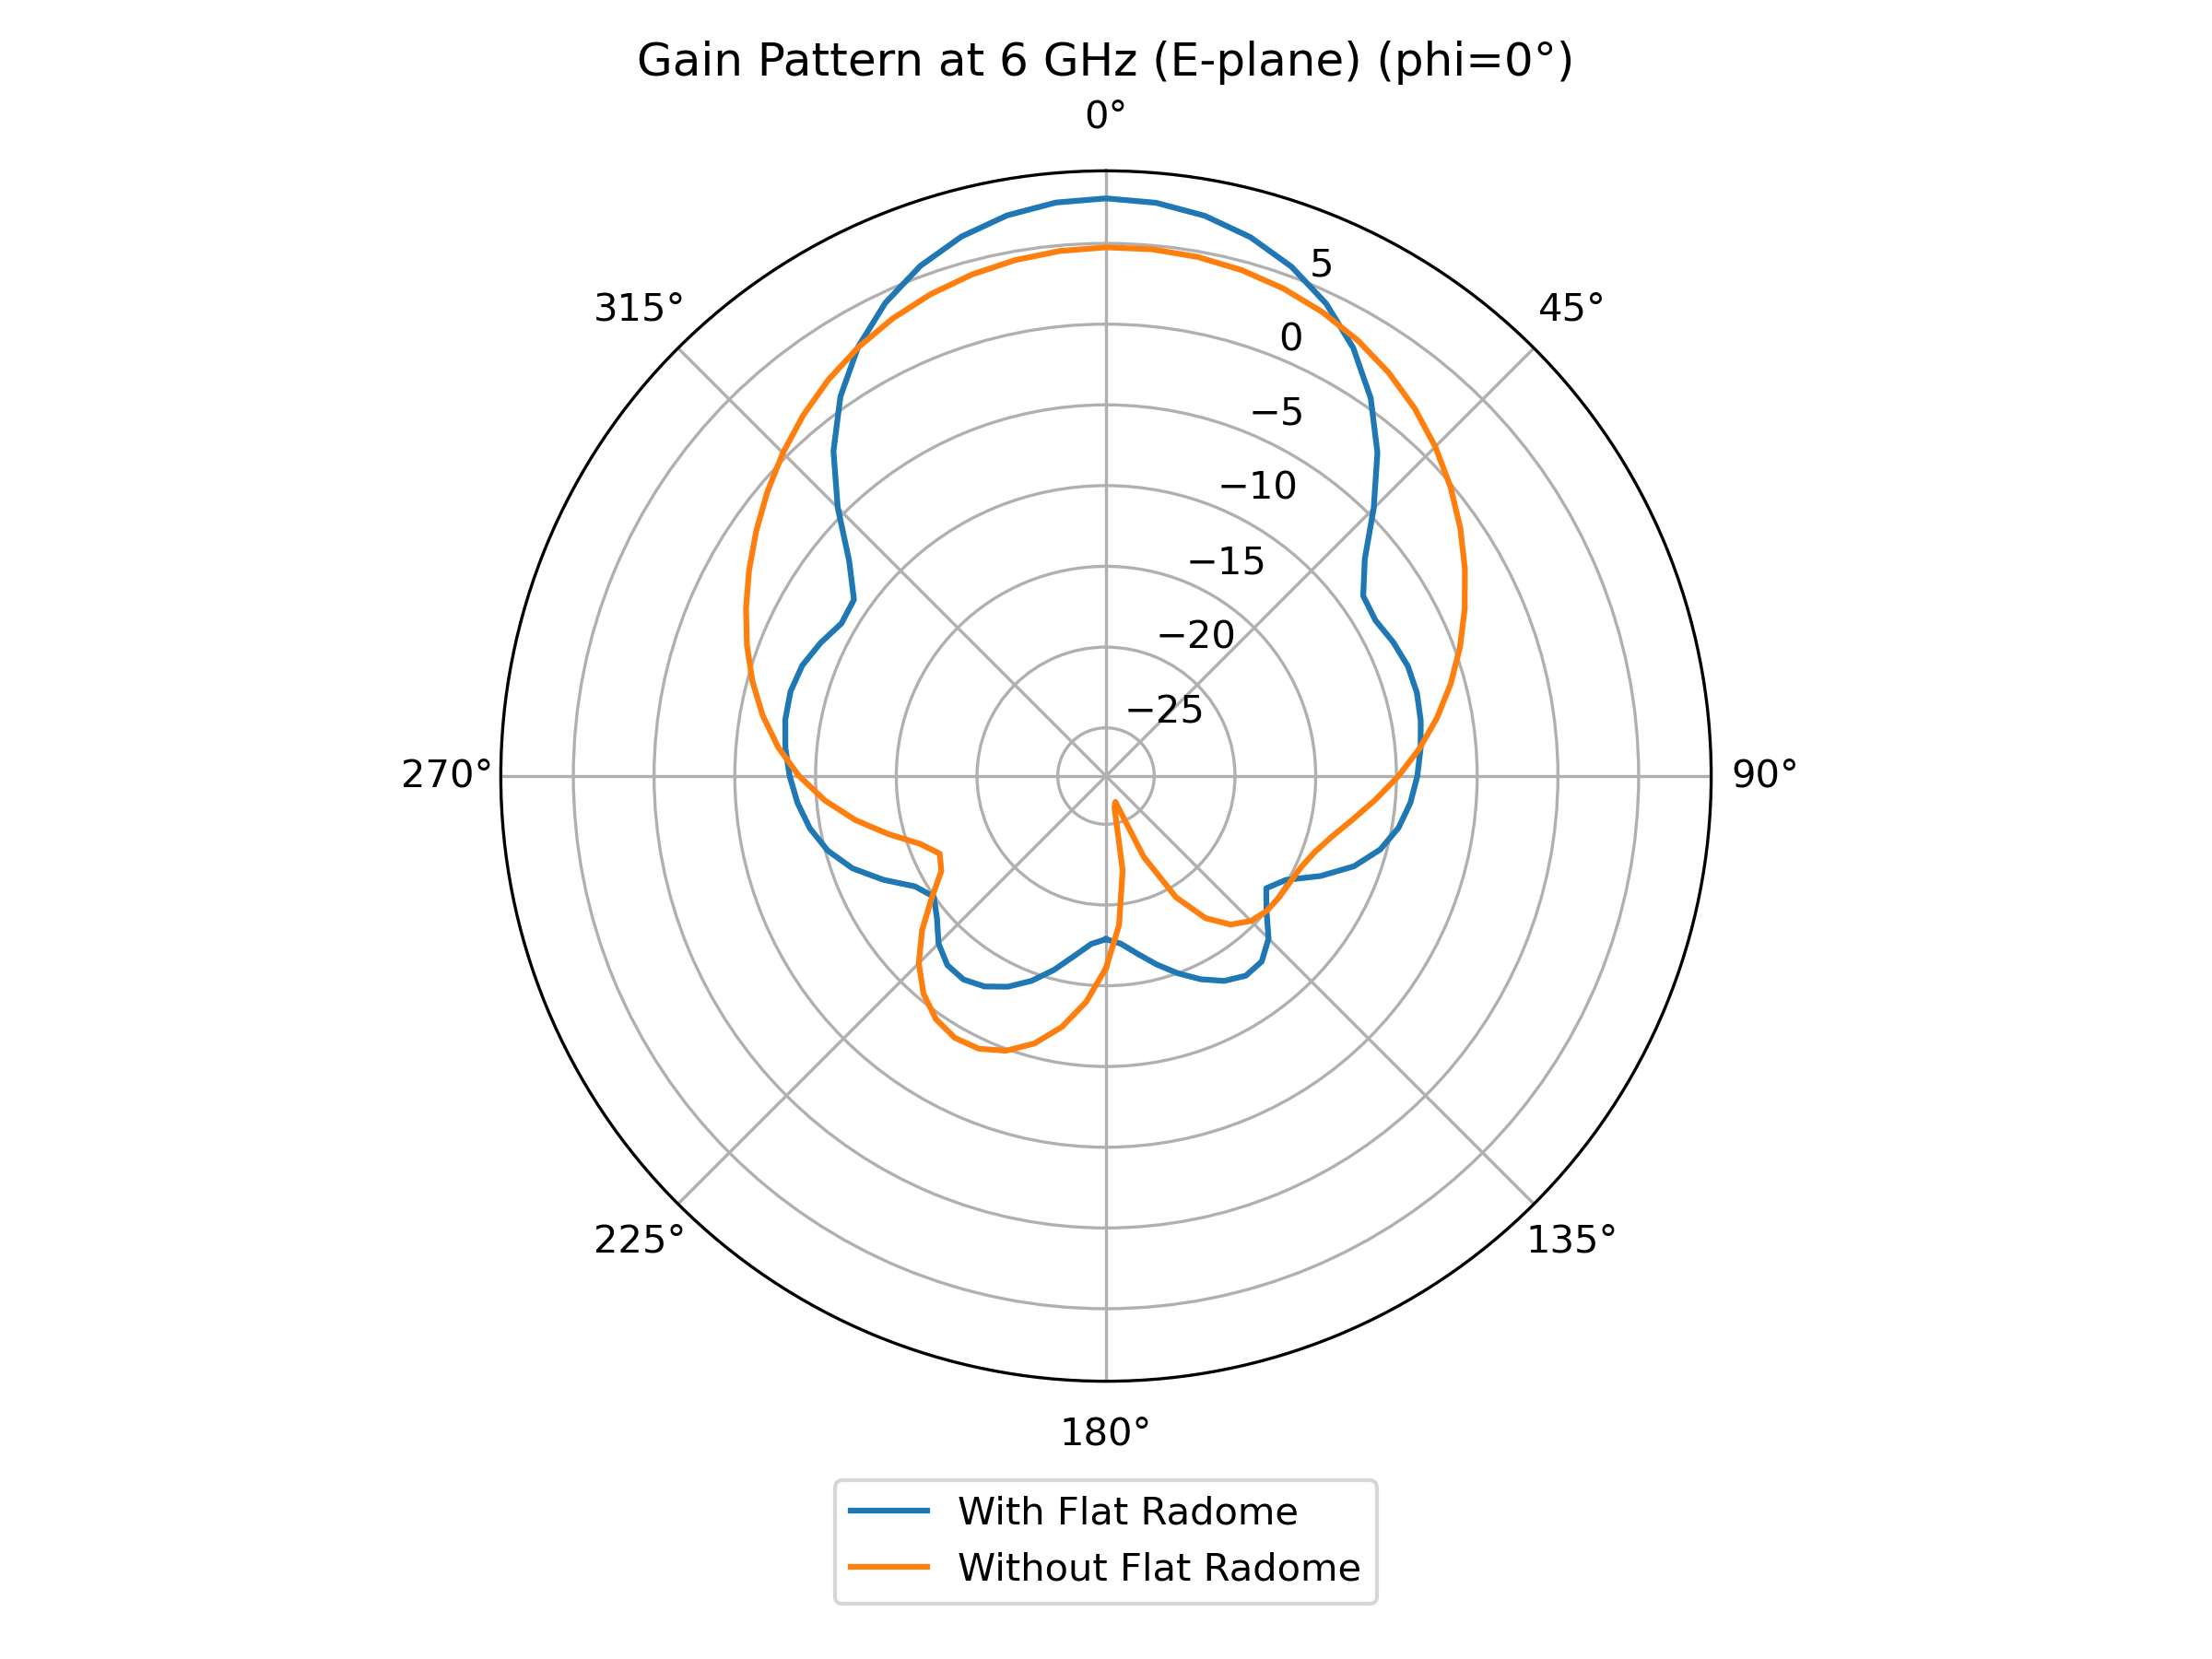
\includegraphics[width=1.0\textwidth]{figures/comparison_flat_radome/gainE_6_GHz.png}
\caption{Simulated gain of the patch antenna with flat radome at 6,GHz.}
\label{fig:res-flat-gainE6}
\end{figure}

At 6 GHz (Figure~\ref{fig:res-flat-gainE6}), which is closer to the antenna's presumed resonance frequency, the gain remains strong and closely matches the free-space case. The peak gain for both "With Radome" (blue line) and "Without Radome" (orange line) is approximately 5 dB. This indicates that the radome design is largely transparent and introduces minimal impact on the antenna's performance near its operating band center.

\begin{figure}[H]
\centering
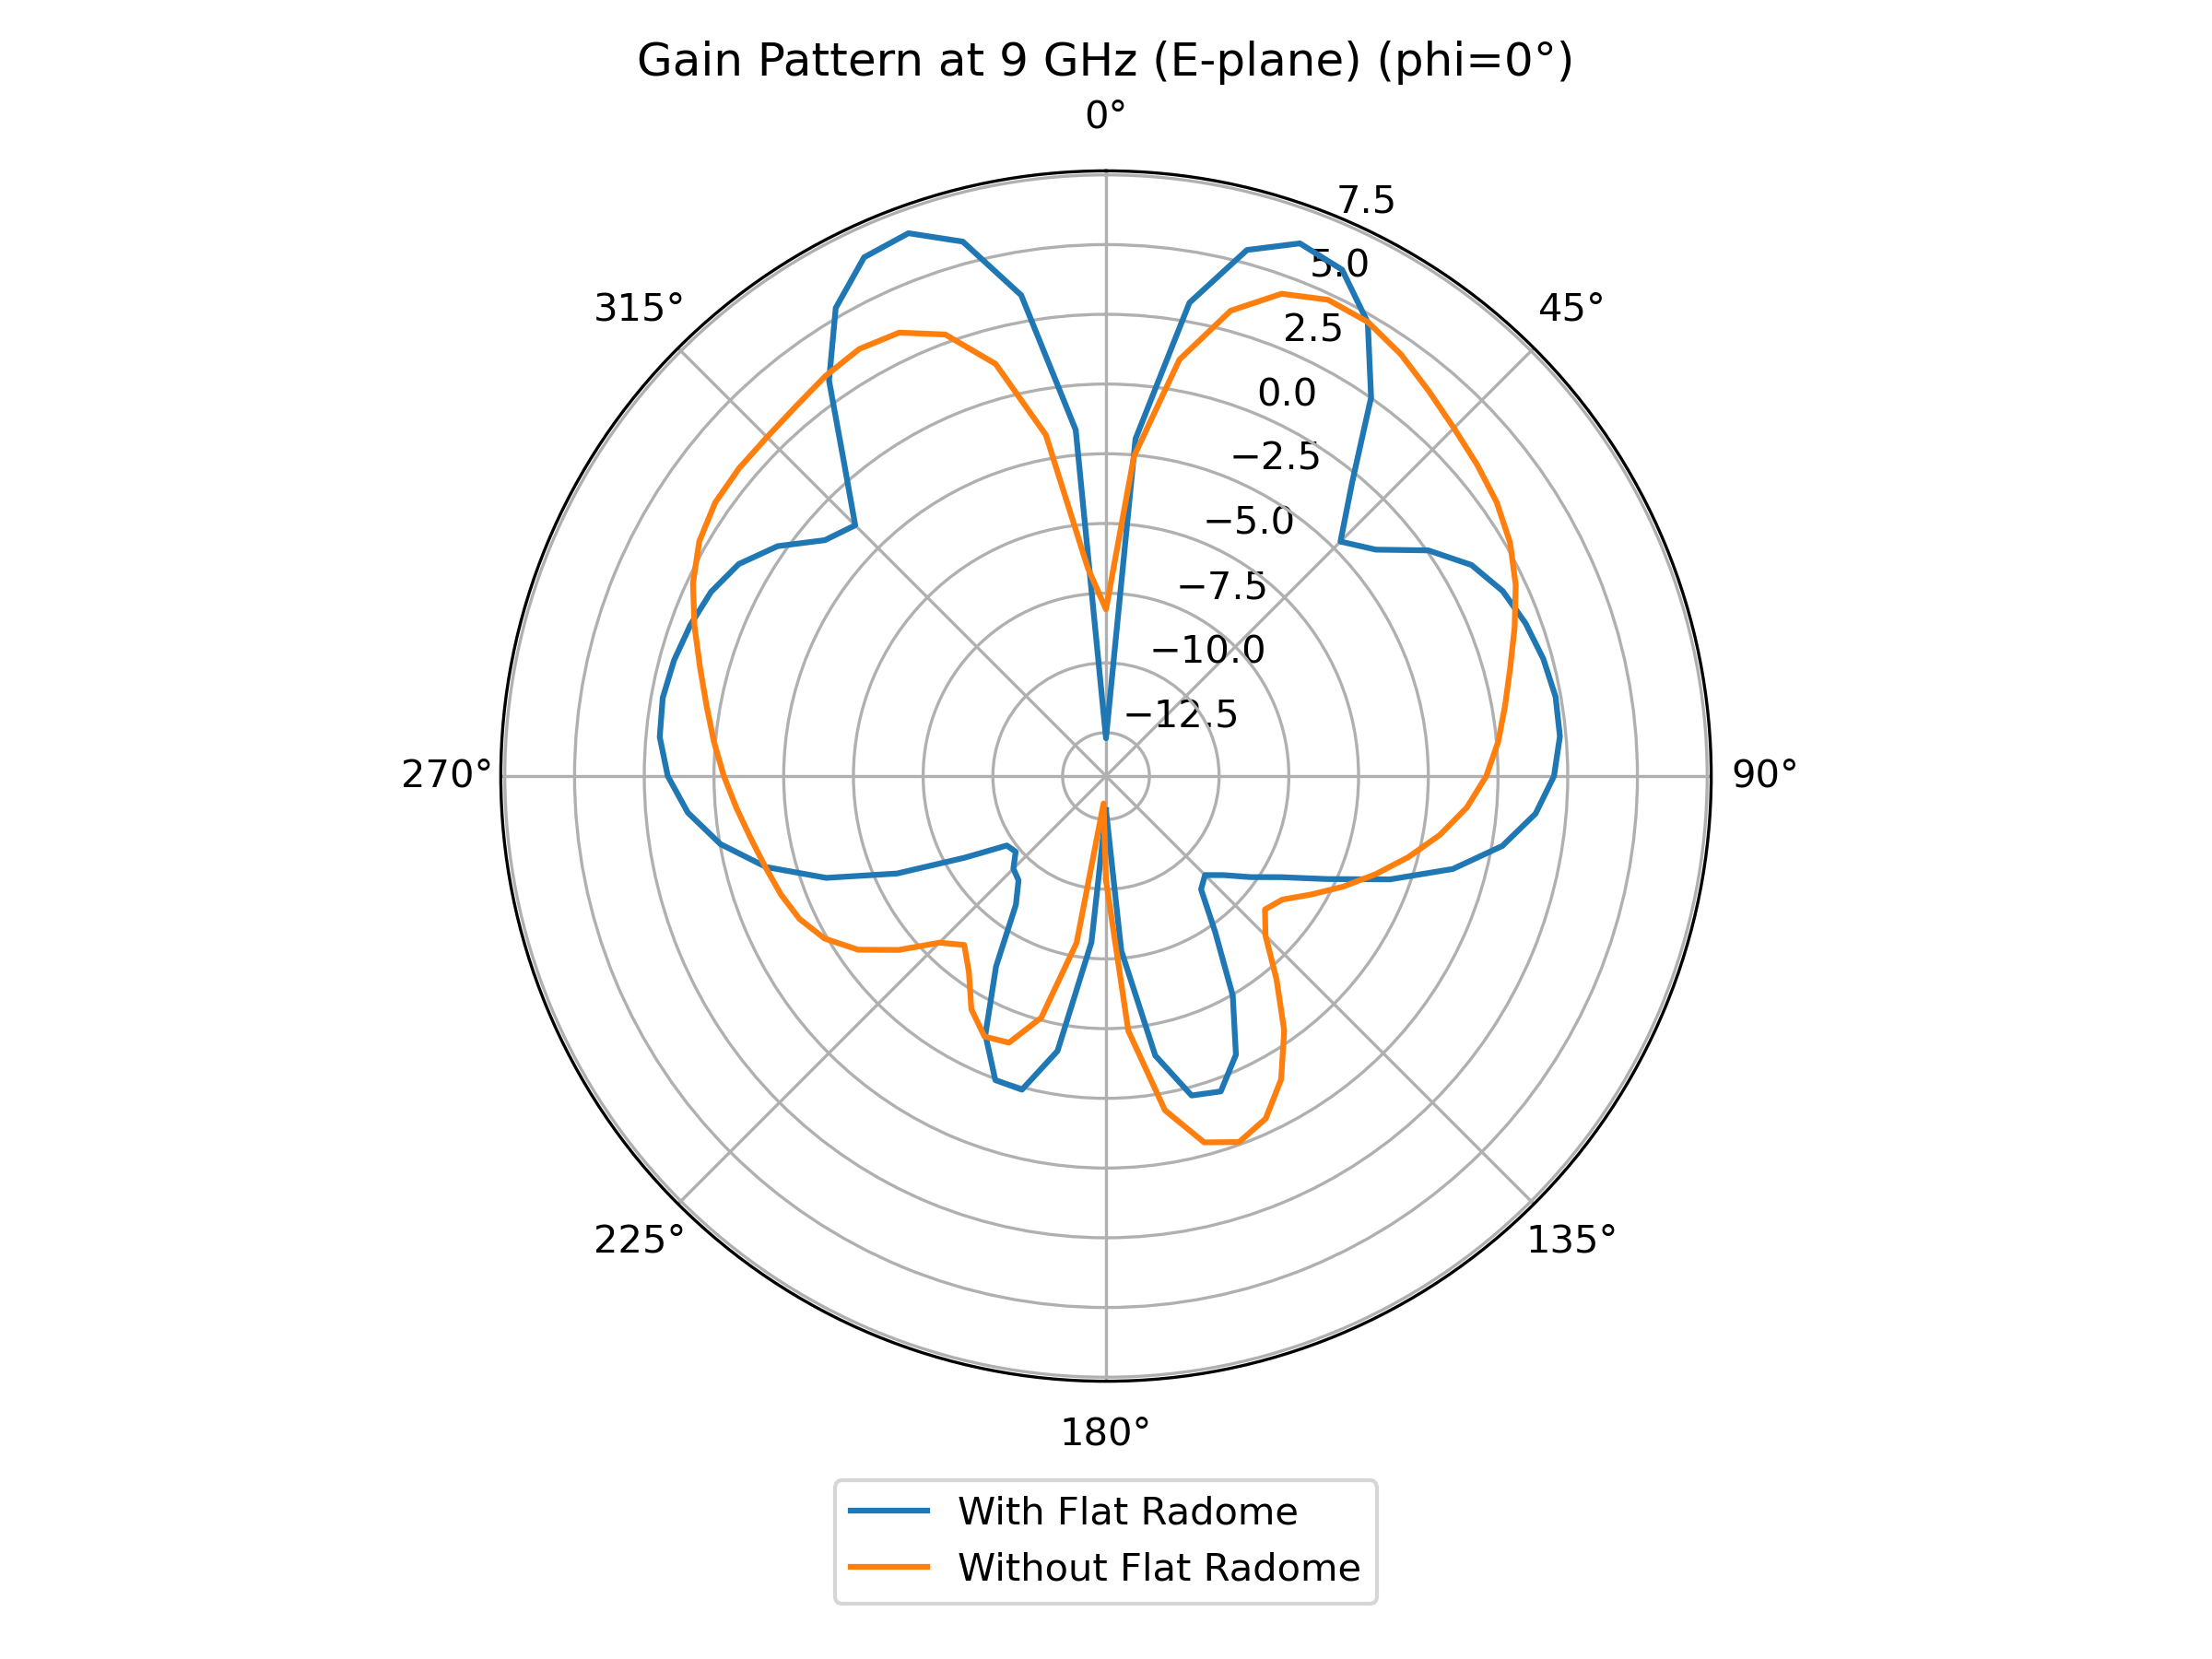
\includegraphics[width=1.0\textwidth]{figures/comparison_flat_radome/gainE_9_GHz.png}
\caption{Simulated gain of the patch antenna with flat radome at 9,GHz.}
\label{fig:res-flat-gainE9}
\end{figure}

Figure~\ref{fig:res-flat-gainE9} shows degradation in gain at the higher frequency end (9 GHz) in the E-plane. The maximum gain with the radome (blue line) is around 5 dB, whereas without the radome (orange line) it is closer to 2.5 dB. The radome causes a increase in the peak gain and also appears to slightly alter the shape of the main lobe, potentially introducing increased side lobe levels at this off-resonant frequency.

\subsection{Gain across Frequencies (H-Plane)}

The H-plane gain patterns (phi=90°) provide insight into the antenna's performance with and without a radome.

\begin{figure}[H]
\centering
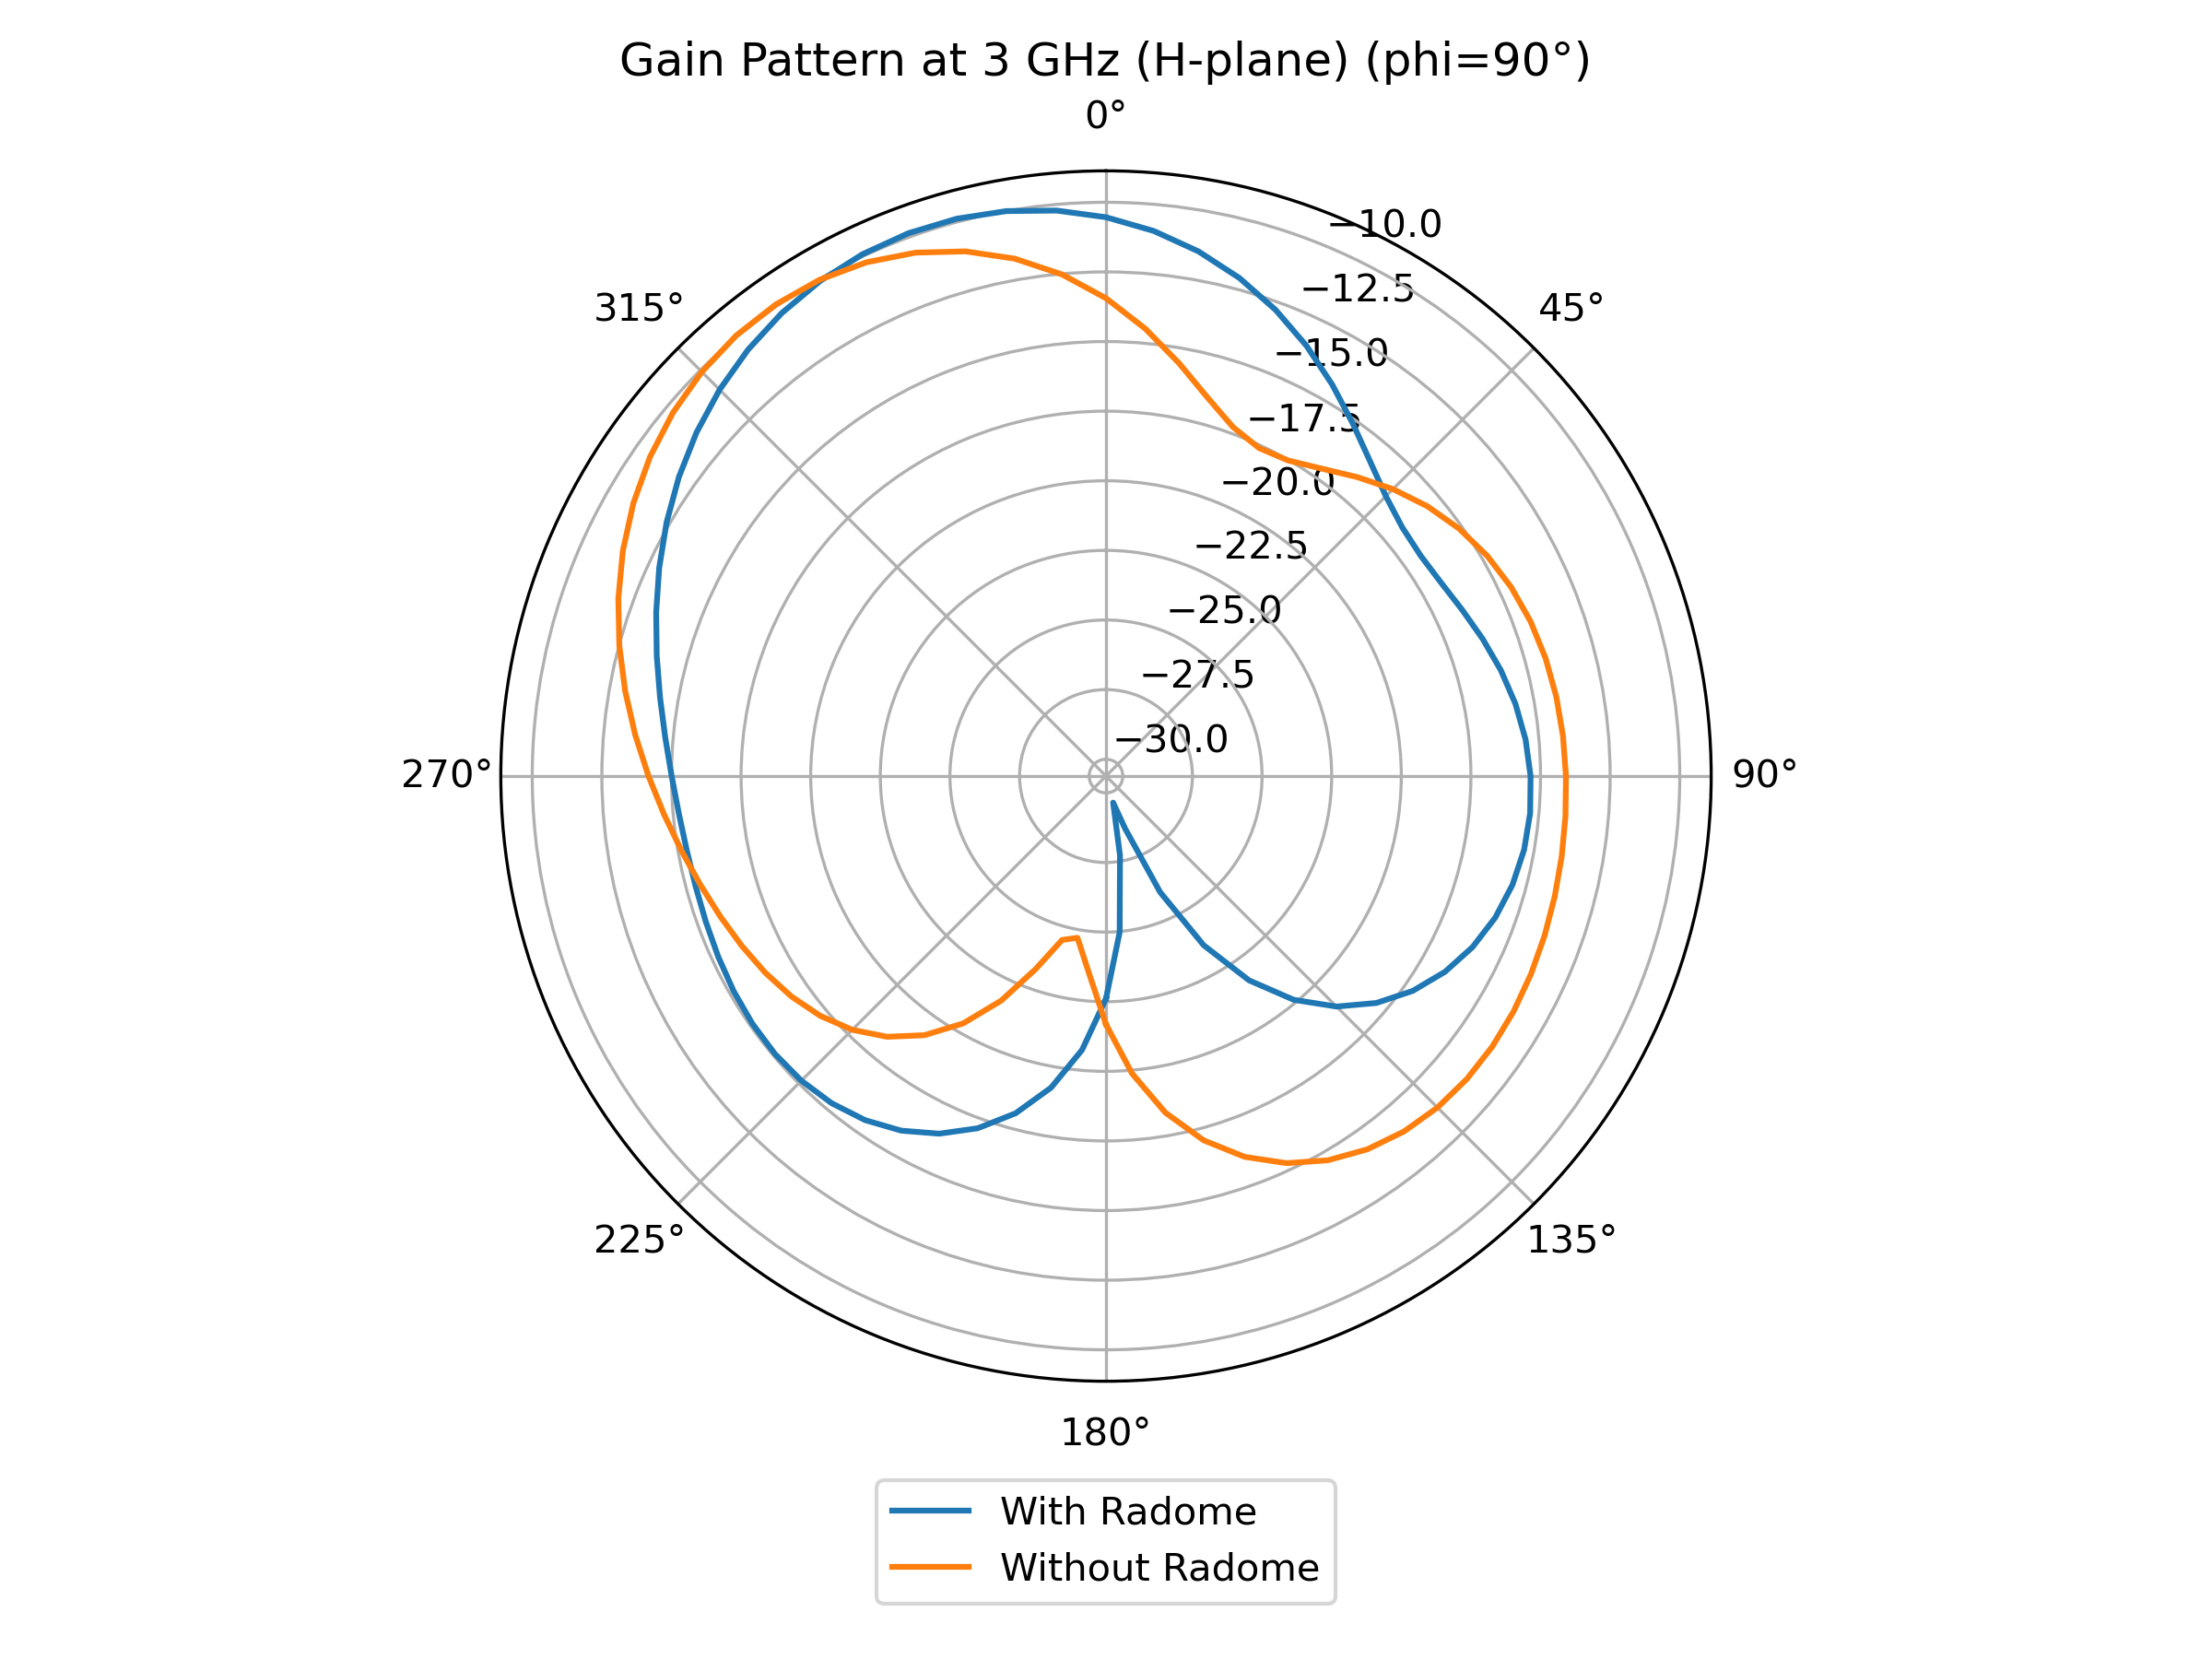
\includegraphics[width=1.0\textwidth]{figures/comparison_flat_radome/gainH_3_GHz.png}
\caption{Simulated gain of the patch antenna with flat radome at 3,GHz.}
\label{fig:res-flat-gainH3}
\end{figure}

Figure~\ref{fig:res-flat-gainH3} illustrates the radiation performance at the lower edge of the band (3 GHz) in the H-plane. Similar to the E-plane at this frequency, the gain of the antenna with the radome (blue line) is reduced compared to the free-space gain (orange line). The peak gain without the radome is around 10 dB, while with the radome, it is approximately -10 dB. The pattern also shows some distortion, indicating a significant negative impact of the radome at this off-resonant frequency.

\begin{figure}[H]
\centering
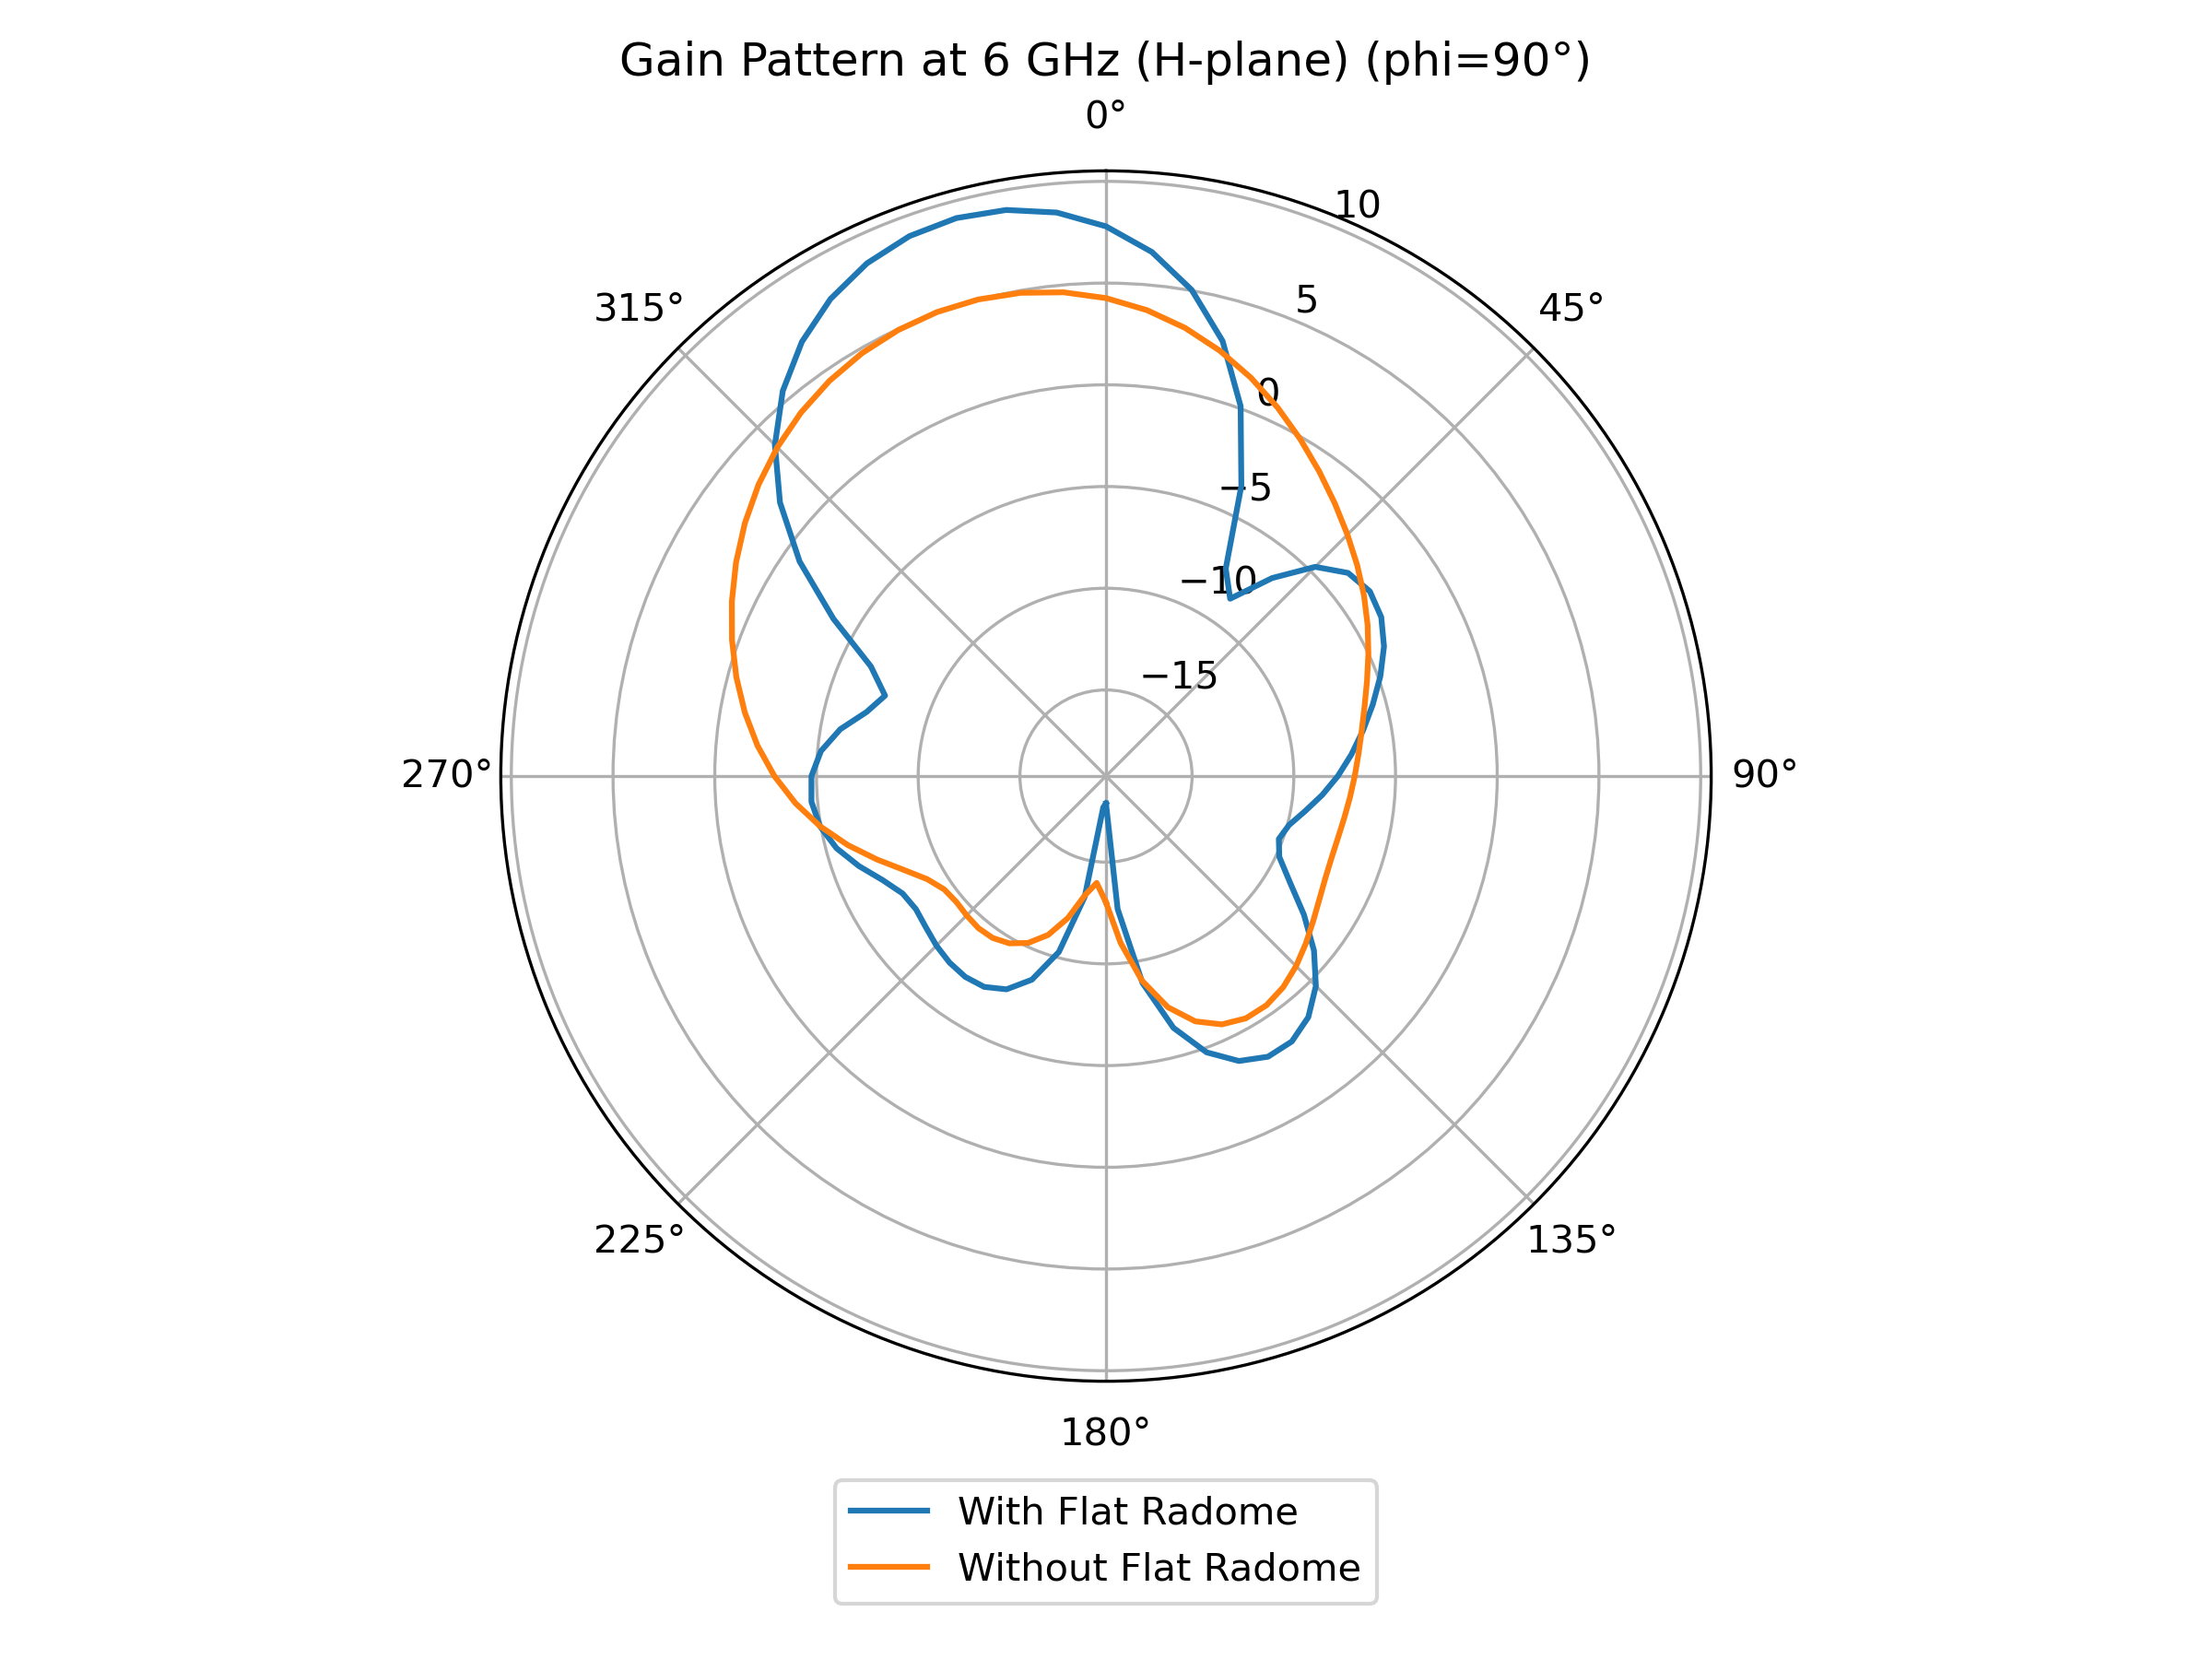
\includegraphics[width=1.0\textwidth]{figures/comparison_flat_radome/gainH_6_GHz.png}
\caption{Simulated gain of the patch antenna with flat radome at 6,GHz.}
\label{fig:res-flat-gainH6}
\end{figure}

At 6 GHz (Figure~\ref{fig:res-flat-gainH6}), close to resonance, the gain in the H-plane remains strong and closely matches the free-space case. The peak gain for both scenarios is approximately about 5 dB, demonstrating the radome's minimal impact and effective transparency at the central operating frequency.

\begin{figure}[H]
\centering
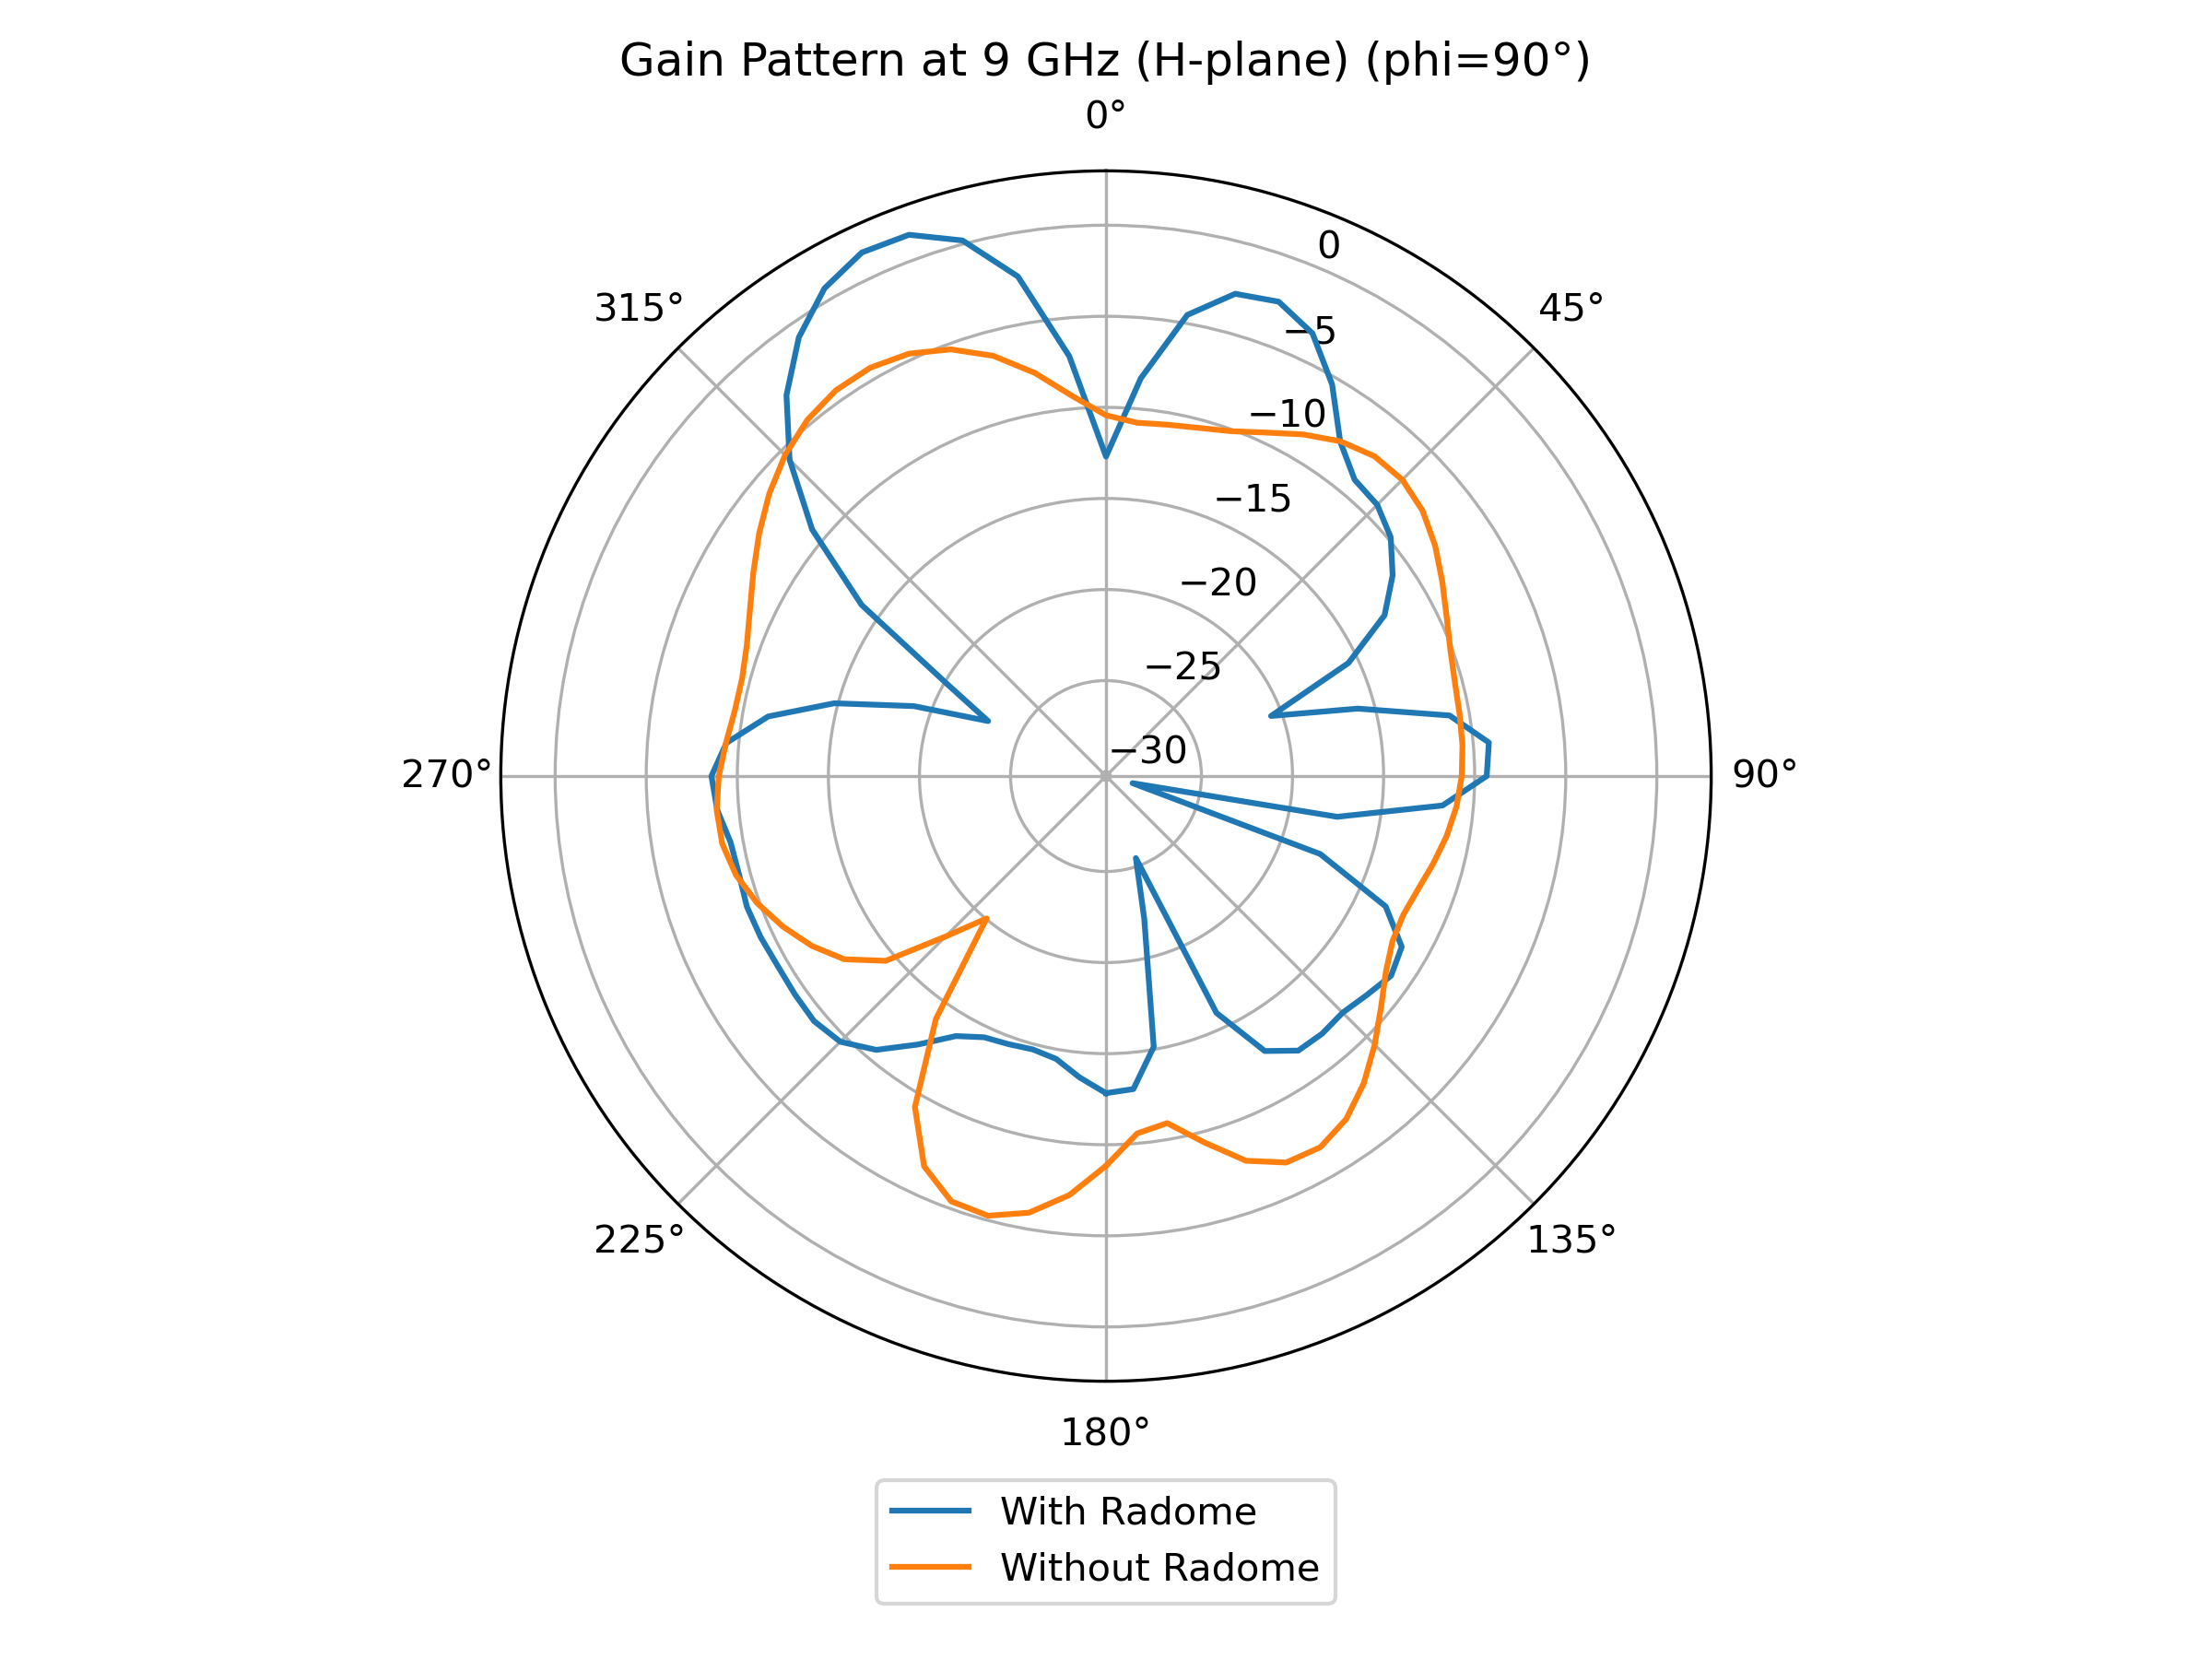
\includegraphics[width=1.0\textwidth]{figures/comparison_flat_radome/gainH_9_GHz.png}
\caption{Simulated gain of the patch antenna with flat radome at 9,GHz.}
\label{fig:res-flat-gainH9}
\end{figure}

Figure~\ref{fig:res-flat-gainH9} shows a more significant degradation in gain at the higher frequency end (9 GHz) in the H-plane. The peak gain without the radome (orange line) is around 0 dB, while with the radome (blue line), it drops to approximately -5 dB. The pattern with the radome also exhibits more pronounced side lobes and a slightly broader main beam compared to the free-space pattern, indicating less optimal performance at this higher off-resonant frequency.

\subsection{Far-Field Patterns}

\begin{figure}[H]
\centering
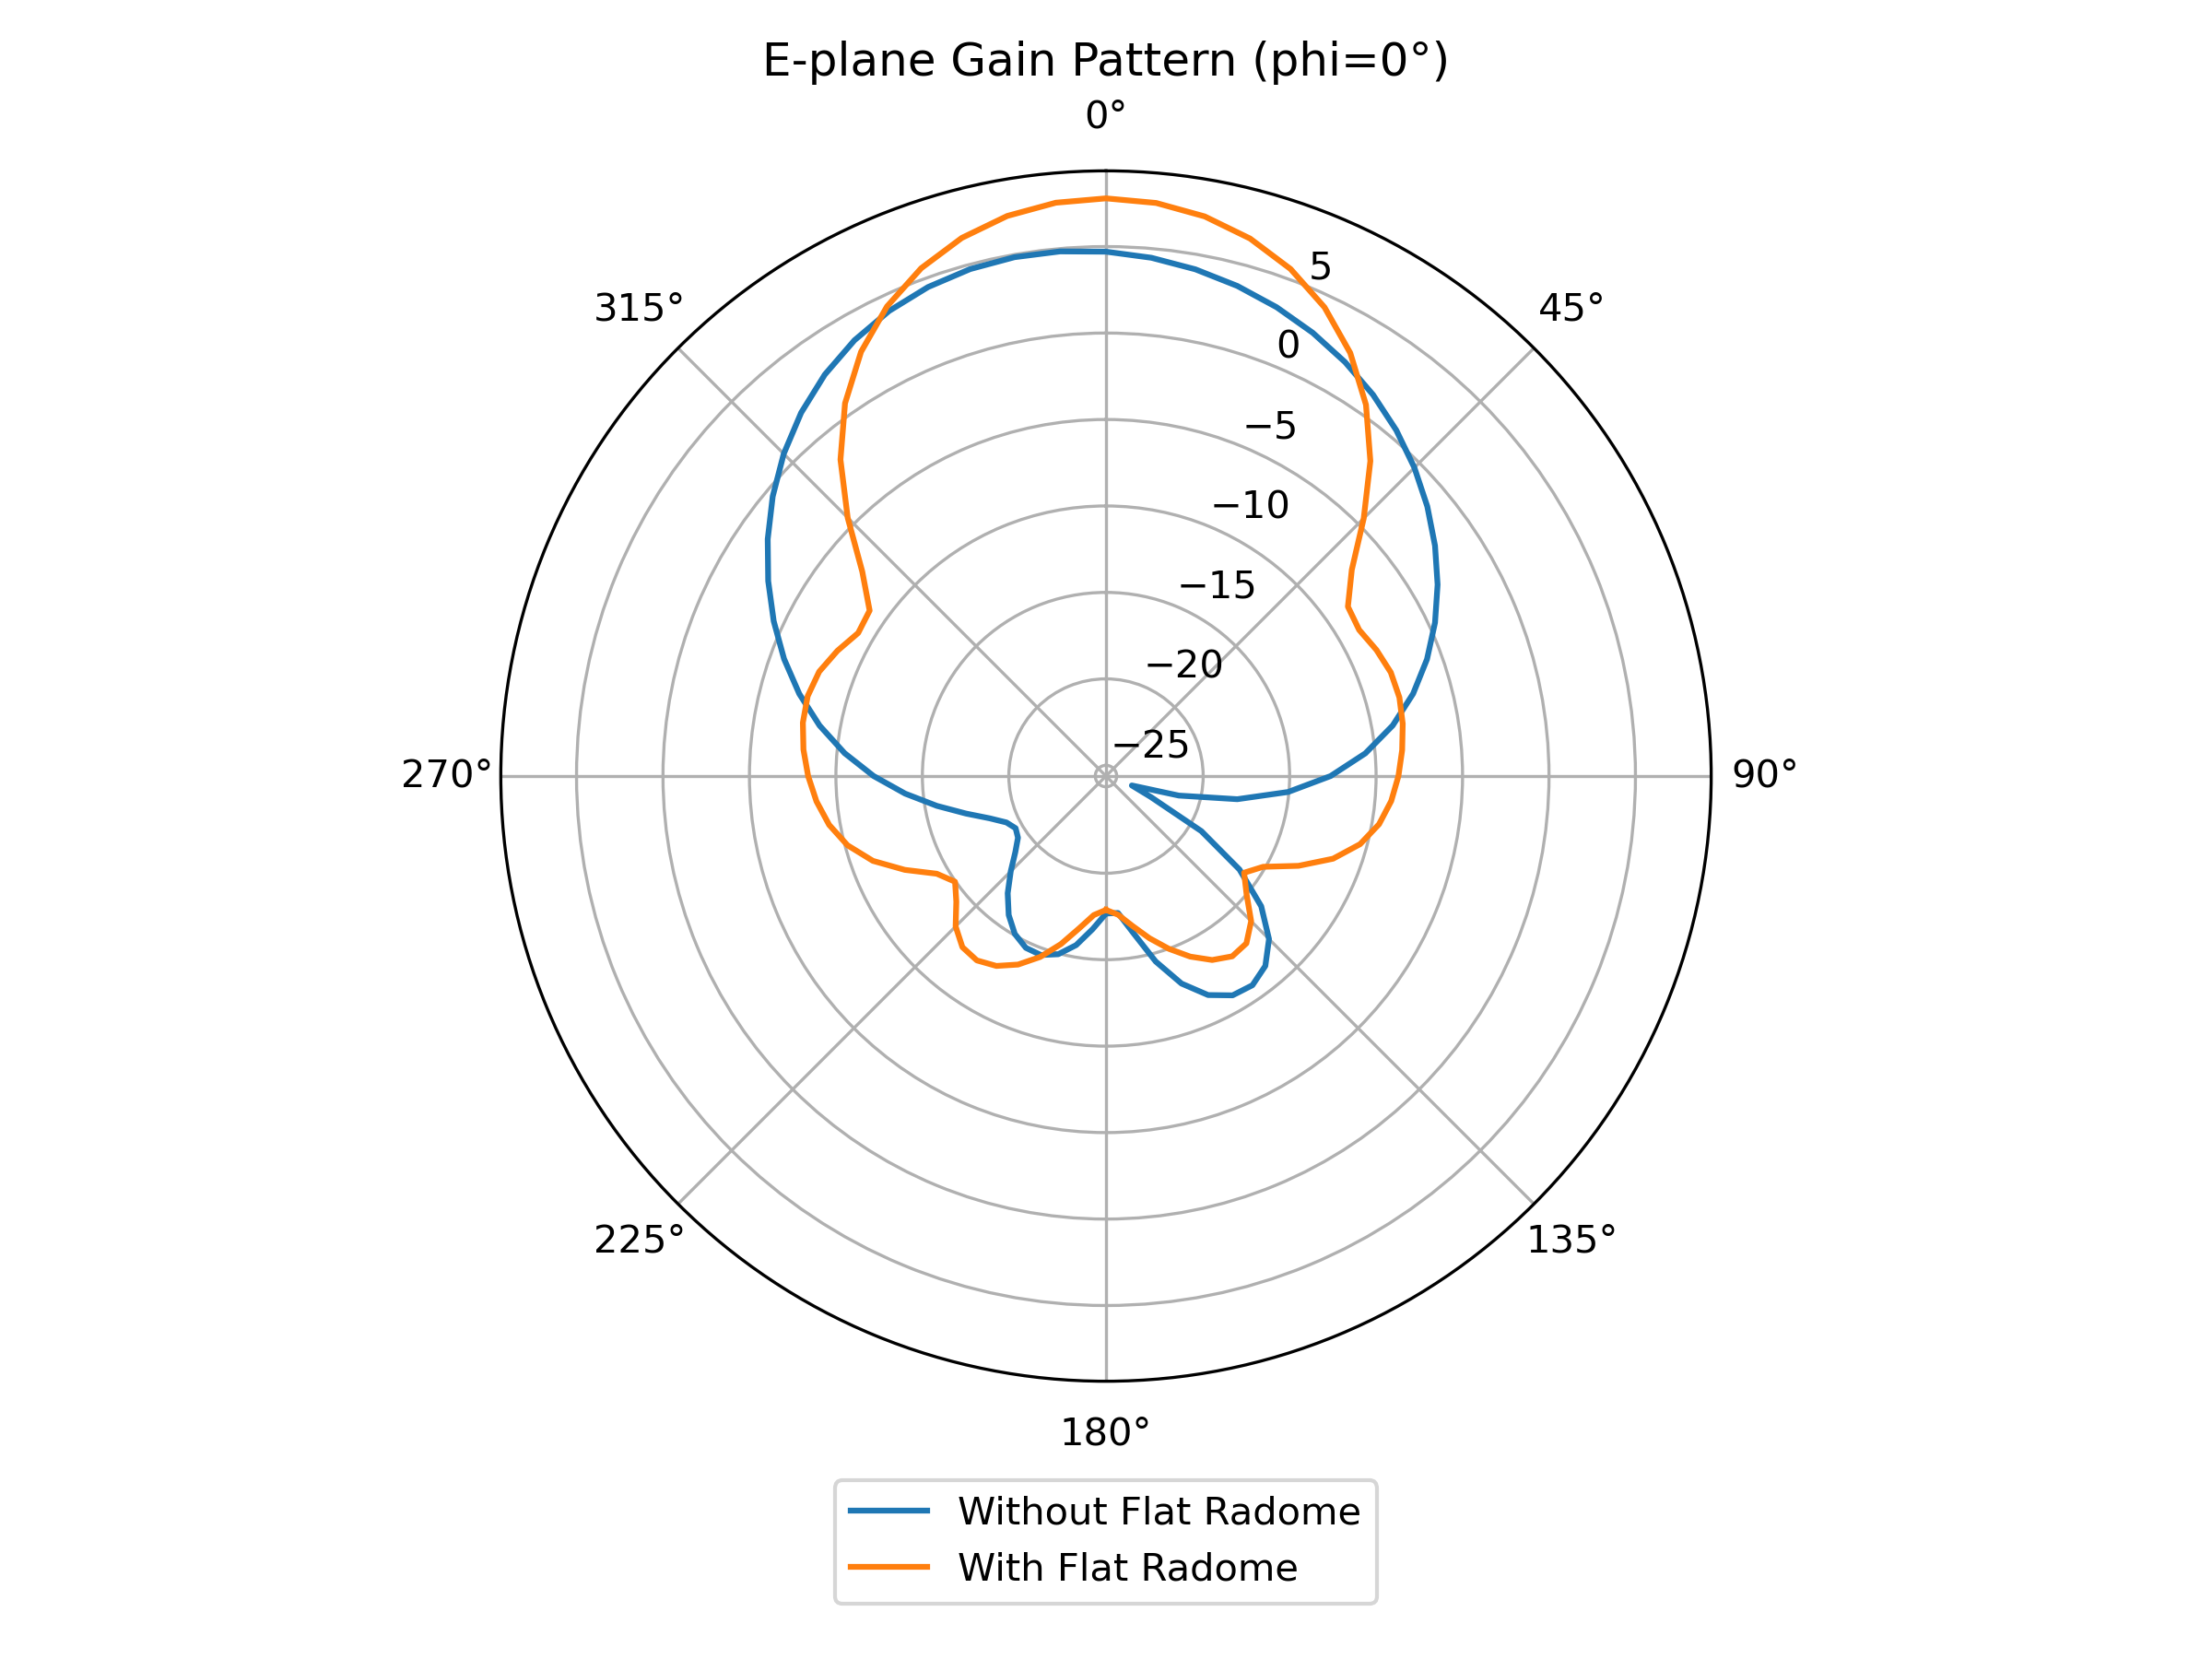
\includegraphics[width=1.0\textwidth]{figures/comparison_flat_radome/gain_E_polar.png}
\caption{Far-field E-plane radiation pattern with flat radome.}
\label{fig:res-flat-eplane}
\end{figure}

The E-plane pattern in Figure~\ref{fig:res-flat-eplane} shows that the overall shape of the radiation pattern is largely maintained with the addition of the radome. However, there is a slight reduction in maximum gain with the radome (orange line) compared to without the radome (blue line) across the main lobe. Additionally, there appears to be a minor increase in the side lobe levels when the radome is present, indicating a slight broadening or less efficient directivity compared to the free-space case.

\begin{figure}[H]
\centering
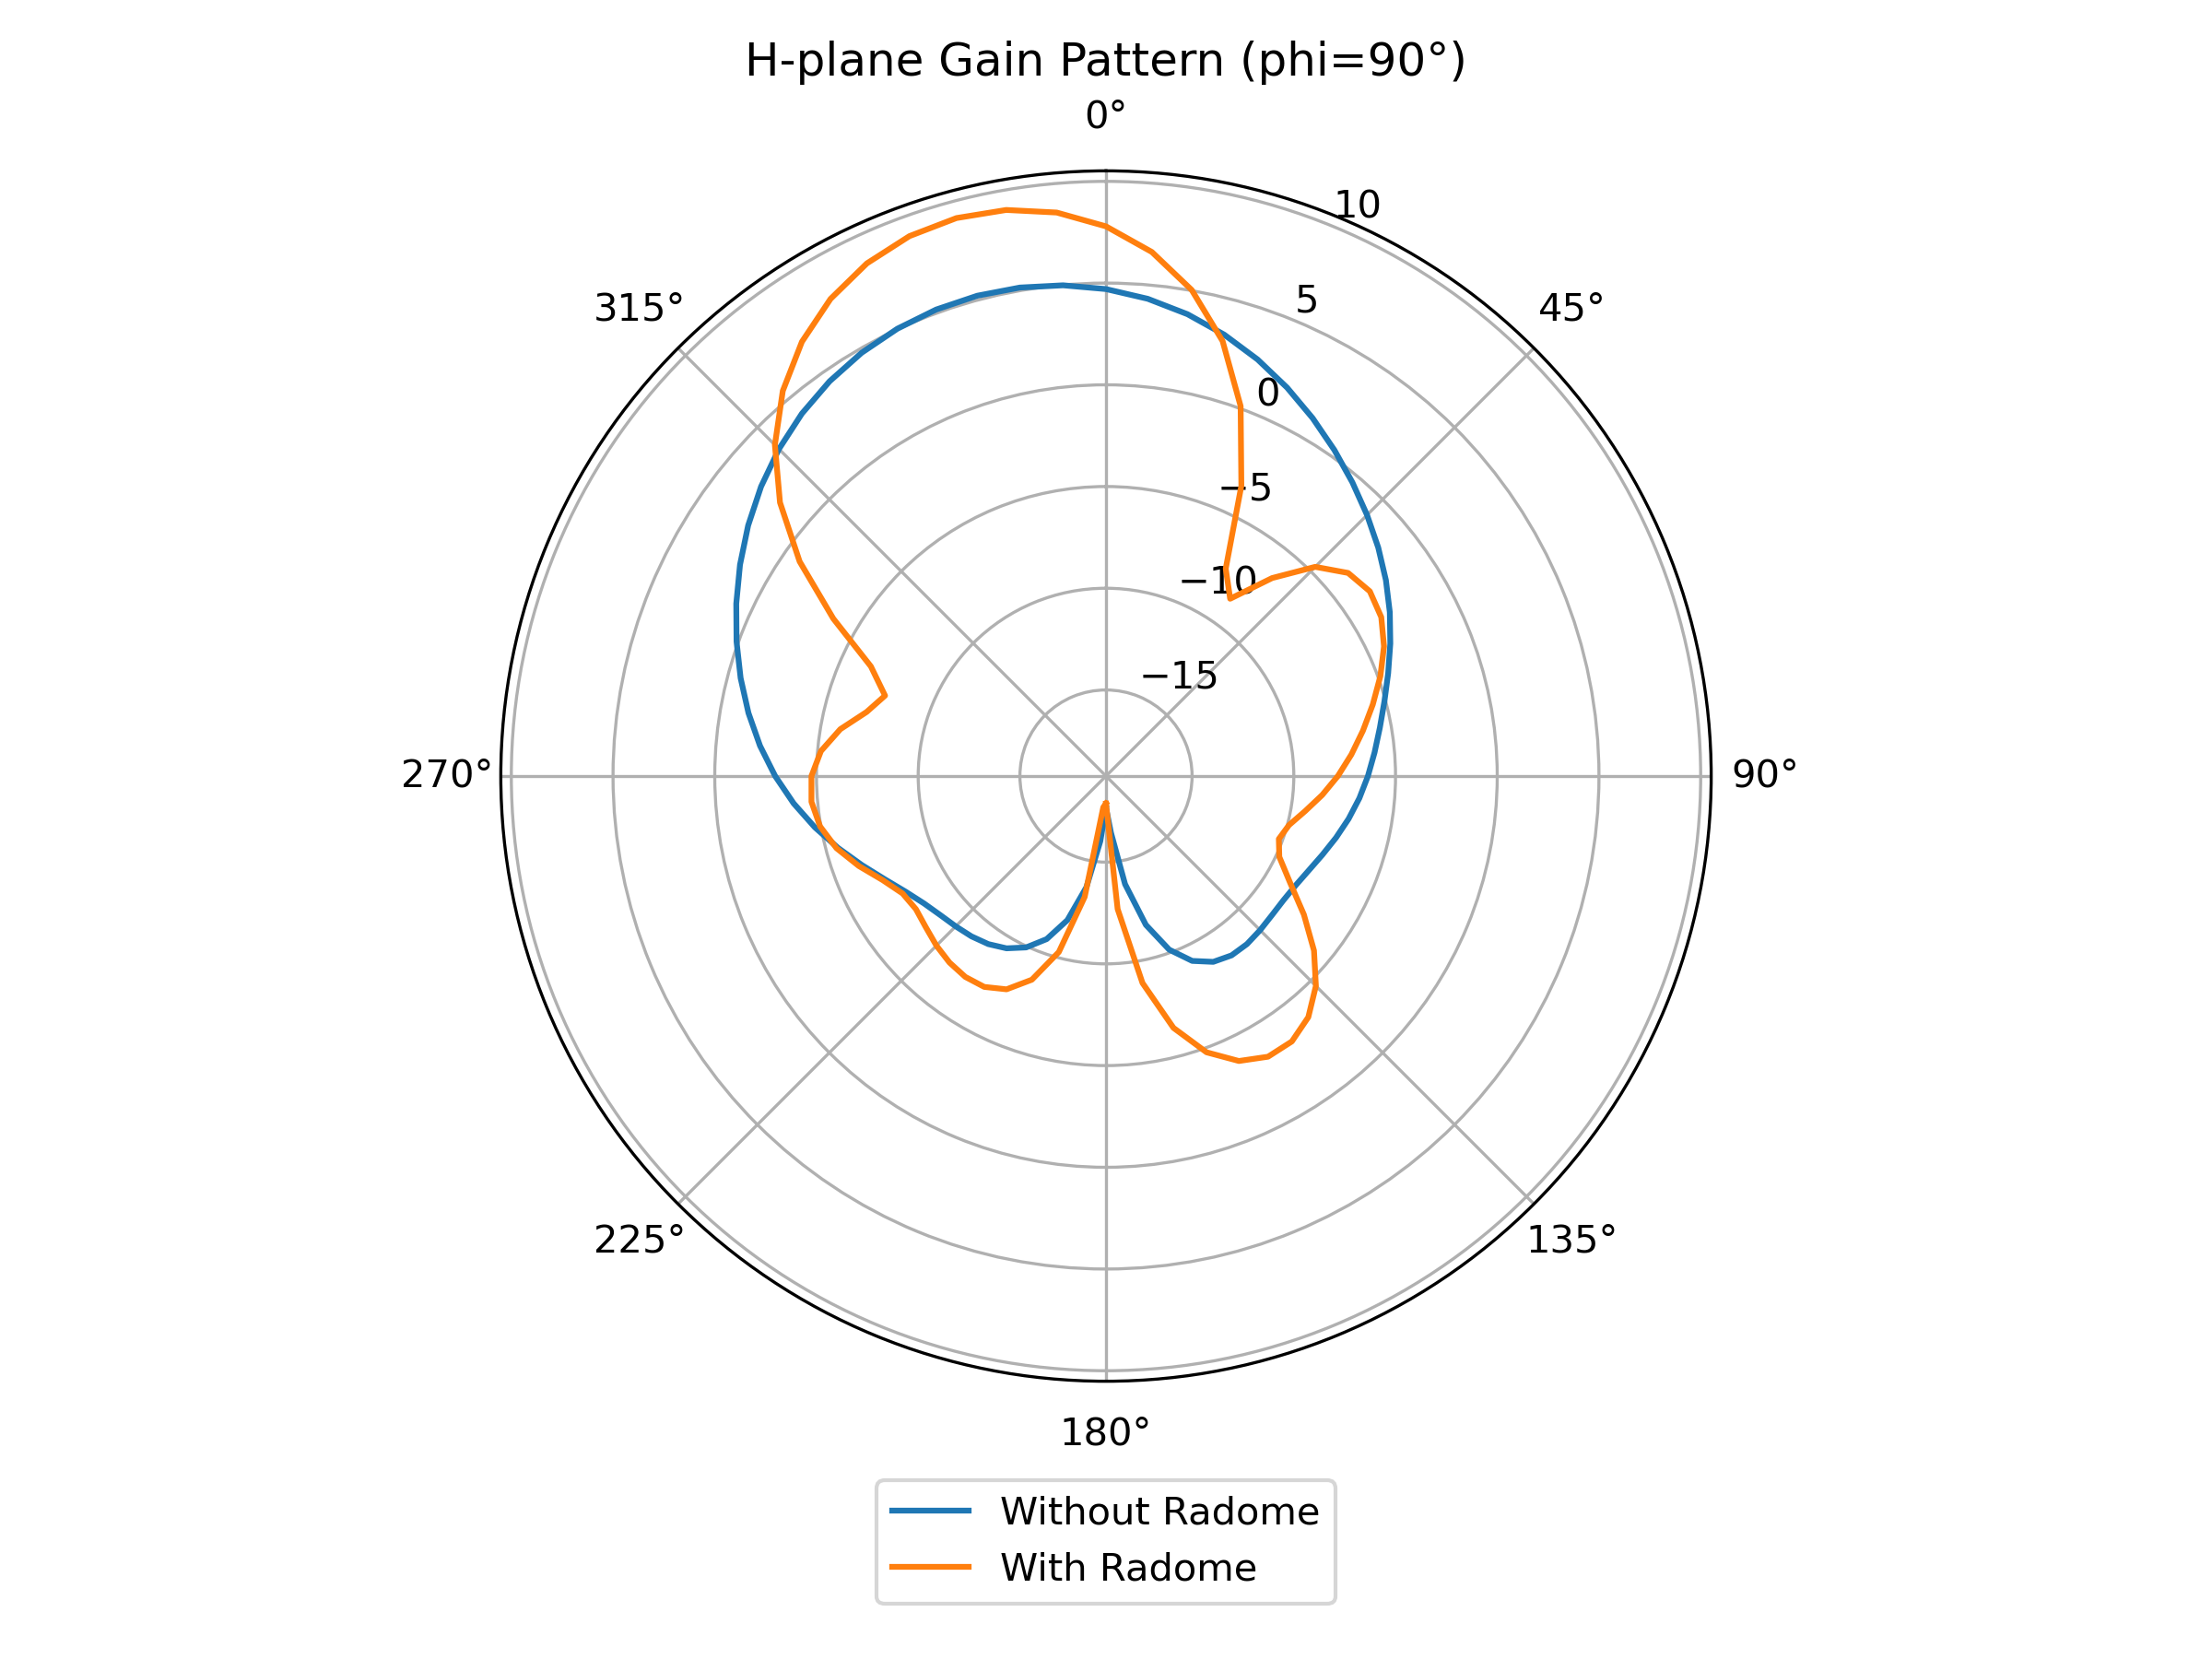
\includegraphics[width=1.0\textwidth]{figures/comparison_flat_radome/gain_H_polar.png}
\caption{Far-field H-plane radiation pattern with flat radome.}
\label{fig:res-flat-hplane}
\end{figure}

In the H-plane (Figure~\ref{fig:res-flat-hplane}), the symmetry of the radiation pattern is generally retained. Similar to the E-plane, there's a slight reduction in the main lobe's peak gain when the radome is present (orange line vs. blue line). Some minor distortions or increased side lobes are also observable, particularly at angles away from the main beam. Overall, the presence of the radome leads to a minor decrease in gain and some pattern distortion in the H-plane.

\subsection{Effect of Radome on \texorpdfstring{$rE$}{rE} Components}

\begin{figure}[H]
    \centering
    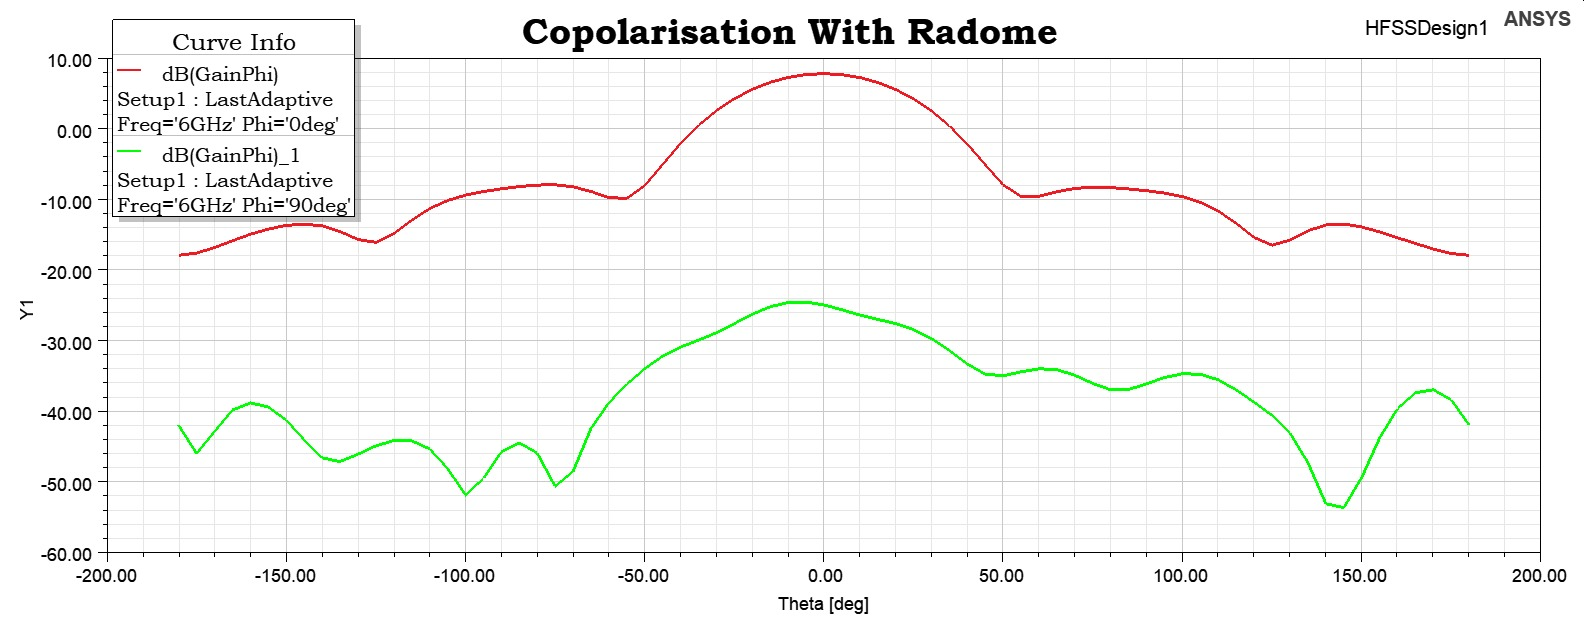
\includegraphics[width=1.0\textwidth]{figures/with_radome/Co.jpeg}
    \caption{Co-polarization response of the patch antenna with flat radome.}
    \label{fig:res-co-radome}
\end{figure}

\begin{figure}[H]
    \centering
    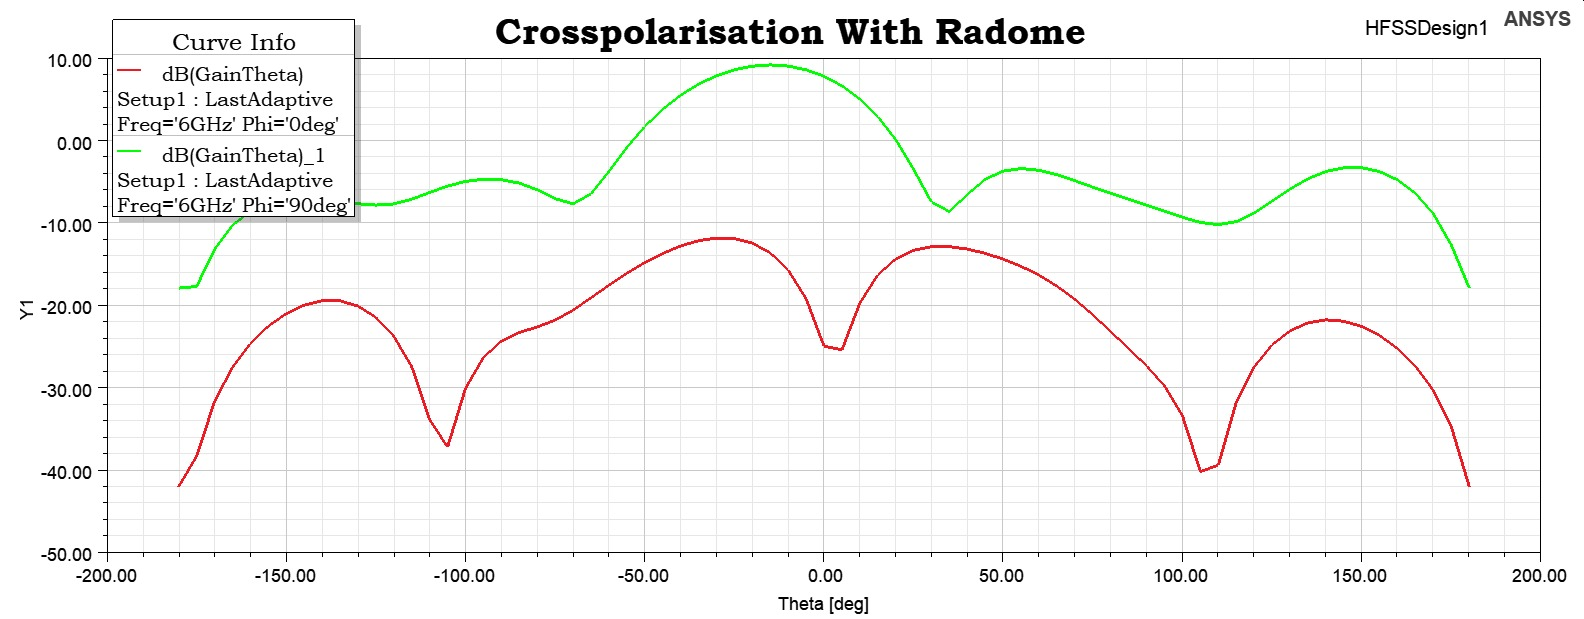
\includegraphics[width=1.0\textwidth]{figures/with_radome/Cross.jpeg}
    \caption{Cross-polarization response of the patch antenna with flat radome.}
    \label{fig:res-cross-radome}
\end{figure}

Figures~\ref{fig:res-co-radome} and \ref{fig:res-cross-radome} present the co-polarization and cross-polarization behavior of the patch antenna when enclosed by a flat radome. Compared to the free-space case, the co-polarized field still maintains a prominent main lobe near the boresight, but with slightly reduced peak gain due to dielectric loading and partial reflection losses introduced by the radome material.

The cross-polarized response shows a marginal increase, particularly at off-boresight angles. This suggests a minor degradation in polarization purity caused by phase distortion and multipath effects within the radome. Nonetheless, the cross-polarization levels remain sufficiently low for most practical applications, indicating that the flat radome preserves acceptable polarization isolation while offering mechanical protection.

% -------------------------------------------------------------------

\newpage
\section*{Summary of Results}

This report presents simulation results for the patch antenna in three configurations:
\begin{itemize}
\item Baseline free-space configuration
\item Optimized feed parameters (parametric sweep)
\item With a flat radome enclosure
\end{itemize}

Performance was evaluated based on return loss, VSWR, gain, directivity, and radiation patterns. The introduction of a flat PMMA radome resulted in:
\begin{itemize}
\item A small frequency shift and increase in VSWR 
\item Mixed impact on gain performance:
\begin{itemize}
\item Significant gain enhancement observed at 3 GHz in both E-plane (Figure \ref{fig:res-flat-gainE3}) and H-plane (Figure \ref{fig:res-flat-gainH3}). This suggests the radome, at this lower frequency, may be acting as a director or through constructive interference, leading to a notable increase in peak gain. For example, in the H-plane at 3 GHz, the gain increases from approximately -10 dB to 10 dB. Similarly, in the E-plane at 3 GHz, it increases from about -10 dB to -8 dB.
\item Near-transparent behavior at 6 GHz (resonant frequency) in both E-plane (Figure \ref{fig:res-flat-gainE6}) and H-plane (Figure \ref{fig:res-flat-gainH6}), where the gain closely matches the free-space performance.
\item Mild gain degradation at 9 GHz (off-resonant frequency) in both E-plane (Figure \ref{fig:res-flat-gainE9}) and H-plane (Figure \ref{fig:res-flat-gainH9}).
\item Overall gain enhancement in the far-field polar plots (Figure \ref{fig:res-flat-eplane} and Figure \ref{fig:res-flat-hplane}), particularly noticeable in the H-plane, where the peak gain with the radome is higher, suggesting a beneficial effect on overall directivity across the depicted pattern.
\end{itemize}
\item Preserved far-field pattern shape with minor beam broadening or side lobe level changes at certain frequencies.
\end{itemize}

\section*{Conclusion}

The simulation results clearly demonstrate the impact of radome enclosures on patch antenna performance. While the free-space antenna shows expected performance, the introduction of a PMMA radome causes measurable shifts in return loss and slight degradation in gain. These results validate the theoretical models and material considerations discussed in previous chapters. The final chapter will summarize the findings, discuss limitations, and propose directions for future work.

\chapter{Conclusion}

This report presented the design, simulation, and analysis of a microstrip patch antenna enclosed within a flat radome structure. The study covered theoretical foundations of antenna radiation, the role of radomes in protecting antenna systems, and the interaction between the antenna and dielectric enclosure.

Patch antennas were chosen due to their low profile, ease of fabrication, and suitability for compact systems. A flat radome configuration was analyzed in detail, focusing on its impact on gain, polarization purity, and far-field radiation characteristics. Simulation results confirmed that the presence of the flat radome introduces measurable but manageable effects on antenna performance. Key parameters such as co- and cross-polarization behavior, beam shape, and gain patterns were evaluated with and without the radome to quantify this influence.

While the project was limited to flat radome geometries, the insights obtained here lay the groundwork for broader investigations into other radome types and materials. The methodology and results can directly inform the design of robust, high-performance antennas for radio astronomy and other applications operating in demanding environmental conditions.

\chapter*{Acknowledgements}
\addcontentsline{toc}{chapter}{Acknowledgements}

I would like to express my sincere gratitude to \textbf{Arjun Ghosh} for his invaluable guidance and support throughout this project. I also thank \textbf{Krittika}, the astronomy club of IIT Bombay, for providing this research opportunity and the necessary resources.  

I am grateful to my project teammates --- \textbf{Sandipan}, \textbf{Dileep}, \textbf{Anvit}, and \textbf{Aleena} --- for their collaboration, dedication, and teamwork. I also acknowledge the project facilitator, \textbf{Aditi Singh}, for helping coordinate and guide the progress of the work.  

Special thanks to my sister, \textbf{Madhumitha}, for generously providing her laptop, which allowed me to run the required simulations. I would like to thank \textbf{Aryan Namboodiri} for engaging discussions and helpful tips that enhanced my understanding, and \textbf{Vibhashree} for assisting me in learning antenna design tools such as HFSS.  

Their collective encouragement and contributions have been instrumental to the progress of this project.


\nocite{*}
\bibliographystyle{unsrt}
\bibliography{bibliography/bibliography.bib}

\end{document}